%% ----------------------------------------------------------------
%% Thesis.tex -- MAIN FILE (the one that you compile with LaTeX)
%% ---------------------------------------------------------------- 

% Set up the document
\documentclass[a4paper, 12pt, oneside]{Thesis}  % Use the "Thesis" style, based on the ECS Thesis style by Steve Gunn
\graphicspath{{Figures/}}  % Location of the graphics files (set up for graphics to be in PDF format)

% Include any extra LaTeX packages required
\usepackage[square, numbers, comma, sort&compress]{natbib}  % Use the "Natbib" style for the references in the Bibliography
\usepackage{verbatim}  % Needed for the "comment" environment to make LaTeX comments
\usepackage{vector}  % Allows "\bvec{}" and "\buvec{}" for "blackboard" style bold vectors in maths
\hypersetup{urlcolor=blue, colorlinks=true}  % Colours hyperlinks in blue, but this can be distracting if there are many links.

%% ----------------------------------------------------------------
\begin{document}
\frontmatter      % Begin Roman style (i, ii, iii, iv...) page numbering

% Set up the Title Page
\title  {Distributed Financial Data Forecaster}
\authors  {\texorpdfstring
            {\href{http://i.cs.hku.hk/~msd15090/index.html}{Wang Youan}}
            {Wang Youan}
            }
\addresses  {\groupname\\\deptname\\\univname}  % Do not change this here, instead these must be set in the "Thesis.cls" file, please look through it instead
\date       {\today}
\subject    {Computer Science}
\keywords   {Artificial Neural Network, Stock Prediction, Apache Spark, Distributed Computing, Technical Indicators, Fundamental Analysis, Data Mining, Machine Learning}

\maketitle
%% ----------------------------------------------------------------

\setstretch{1.5}  % It is better to have smaller font and larger line spacing than the other way round

% Define the page headers using the FancyHdr package and set up for one-sided printing
\fancyhead{}  % Clears all page headers and footers
\rhead{\thepage}  % Sets the right side header to show the page number
\lhead{}  % Clears the left side page header

\pagestyle{fancy}  % Finally, use the "fancy" page style to implement the FancyHdr headers

%% ----------------------------------------------------------------
% Declaration Page required for the Thesis, your institution may give you a different text to place here
\Declaration{

\addtocontents{toc}{\vspace{1em}}  % Add a gap in the Contents, for aesthetics

I, WANG Youan, declare that this thesis titled, 'Distributed Financial Data Forecaster' and the work presented in it are my own. I confirm that:

\begin{itemize} 
\item[\tiny{$\blacksquare$}] This work was done wholly or mainly while in candidature for a degree at this University.
 
\item[\tiny{$\blacksquare$}] Where any part of this thesis has previously been submitted for a degree or any other qualification at this University or any other institution, this has been clearly stated.
 
\item[\tiny{$\blacksquare$}] Where I have consulted the published work of others, this is always clearly attributed.
 
\item[\tiny{$\blacksquare$}] Where I have quoted from the work of others, the source is always given. With the exception of such quotations, this thesis is entirely my own work.
 
\item[\tiny{$\blacksquare$}] I have acknowledged all main sources of help.
 
\item[\tiny{$\blacksquare$}] Where the thesis is based on work done by myself jointly with others, I have made clear exactly what was done by others and what I have contributed myself.
\\
\end{itemize}
 
 
Signed:\\
\rule[1em]{25em}{0.5pt}  % This prints a line for the signature
 
Date:\\
\rule[1em]{25em}{0.5pt}  % This prints a line to write the date
}
\clearpage  % Declaration ended, now start a new page

%% ----------------------------------------------------------------
% The "Funny Quote Page"
\pagestyle{empty}  % No headers or footers for the following pages

\null\vfill
% Now comes the "Funny Quote", written in italics
\textit{``Write a funny quote here.''}

\begin{flushright}
If the quote is taken from someone, their name goes here
\end{flushright}

\vfill\vfill\vfill\vfill\vfill\vfill\null
\clearpage  % Funny Quote page ended, start a new page
%% ----------------------------------------------------------------

% The Abstract Page
\addtotoc{Abstract}  % Add the "Abstract" page entry to the Contents
\abstract{
\addtocontents{toc}{\vspace{1em}}  % Add a gap in the Contents, for aesthetics

This study is to apply different data mining,
}\\
\smallskip
{\bf Keywords:} Artificial Neural Network, Apache Spark, Distributed Computing, Technical Indicators, Fundamental Analysis, Data Mining, Machine Learning
\clearpage  % Abstract ended, start a new page
%% ----------------------------------------------------------------

\setstretch{1.5}  % Reset the line-spacing to 1.3 for body text (if it has changed)

% The Acknowledgements page, for thanking everyone
\acknowledgements{
\addtocontents{toc}{\vspace{1em}}  % Add a gap in the Contents, for aesthetics

The acknowledgements and the people to thank go here, don't forget to include your project advisor\ldots

}
\clearpage  % End of the Acknowledgements
%% ----------------------------------------------------------------

\pagestyle{fancy}  %The page style headers have been "empty" all this time, now use the "fancy" headers as defined before to bring them back


%% ----------------------------------------------------------------
\lhead{\emph{Contents}}  % Set the left side page header to "Contents"
\tableofcontents  % Write out the Table of Contents

%% ----------------------------------------------------------------
\lhead{\emph{List of Figures}}  % Set the left side page header to "List if Figures"
\listoffigures  % Write out the List of Figures

%% ----------------------------------------------------------------
\lhead{\emph{List of Tables}}  % Set the left side page header to "List of Tables"
\listoftables  % Write out the List of Tables

%% ----------------------------------------------------------------
% \setstretch{1.5}  % Set the line spacing to 1.5, this makes the following tables easier to read
\clearpage  % Start a new page
\lhead{\emph{Abbreviations}}  % Set the left side page header to "Abbreviations"
\listofsymbols{ll}  % Include a list of Abbreviations (a table of two columns)
{
% \textbf{Acronym} & \textbf{W}hat (it) \textbf{S}tands \textbf{F}or \\
\textbf{ANN} & \textbf{A}rtificial \textbf{N}eural \textbf{N}etwork \\

}

%% ----------------------------------------------------------------
% End of the pre-able, contents and lists of things
% Begin the Dedication page

% \setstretch{1.5}  % Return the line spacing back to 1.3

\pagestyle{empty}  % Page style needs to be empty for this page
\dedicatory{For/Dedicated to/To my\ldots}

\addtocontents{toc}{\vspace{2em}}  % Add a gap in the Contents, for aesthetics


%% ----------------------------------------------------------------
\mainmatter	  % Begin normal, numeric (1,2,3...) page numbering
\pagestyle{fancy}  % Return the page headers back to the "fancy" style

% Include the chapters of the thesis, as separate files
% Just uncomment the lines as you write the chapters

\chapter{Introduction} 

\section{Problem Statement}

It is human beings' common goal to make life easier and more comfortable. Wealth can bring help to achieve this goal, and investment on stock can help people to gain wealth quickly. As a result, many research works have been done on market analysis.\par 

However, as a very complex (non-linear) and volatile system with many factors (such as companies' performance, domestic economies, festivals, seasons, etc.)\cite{chen1986economic}, stock market is difficult to be precisely predicted. Which makes investors and researchers headache, those factors usually have relationship with each other, and they will keep changing all the time. Hence, investors and fund manager must maintain real-time monitoring of market behavior and take right factors into consideration, so as to make the right trading decision.\par

Is stock price movement really predictable? How to measure the predict performance of given method? As those indicators of market keep changing every time, how can we keep tracking of them timely for many stocks? As calculating so many parameters is really demanding, but those high performance server is very expensive, can we utilize distributed computing to calculate those? With the development of machine learning, computer now can learn some human knowledge (like Alpha Go versus Lee Sedol), can them learn to predict stock price?

\section{Objectives}

This study is to answer the above problems. Target market is Hong Kong Stock Exchange Market. Objects is to find a good method to predict HSI stock price changes through testing on different machine learning algorithms (includes Linear Regression, Neural Network, Random Forest). Apart from using single learning methods, this study also tries to combine two machine learning methods to do that predict, which use one to predict how much a stock price changes and another to forecast what direction the stock price will change (up or down). 

\section{The Dataset}
Most of historical stock information are collected from Yahoo Finance (http://finance.yahoo.com), HIBOR are downloaded from the Hong Kong Association of Banks (HKAB) website, its url is http://www.hkab.org.hk/. Other data are collected through Quandl (https://www.quandl.com/)

\section{Success Criteria}
The purpose of the thesis is to find a stock price prediction system that can be applied as an assistant tool for investors in HKEX. Thus, the core research problem is which algorithm can make the best prediction. Several performance criteria (e.g. MSE, MAPE, details can be found in Appendix A) are used to measure these learning method.


\section{Structure}


This thesis follows the below structure\par
\begin{itemize}
	\item Chapter 1 briefly introduces the problems and shows the objective of this study.
	\item Chapter~\ref{ch:review} reviews previous works one this subject.
	\item Chapter 3 to 7 discuss the research methodology. Chapter~\ref{ch:market} shows understanding to the financial market, and talks about the reason of parameters chosen; Chapter~\ref{ch:mining} discusses data processing method, includes data normalization and deduction; Chapter \ref{ch:machine} introduces those machine learning methods used in this projects; Chapter~\ref{ch:spark} is about basics of Spark; Chapter~\ref{ch:system} gives the design and workflow of prediction system.
	\item Chapter 8 to 10 is about results. Chapter 8 introduces testing environment; Chapter 9 shows testing results of different learning method; Chapter 10 compares running performance of distributed and non-distributed method.
	\item Chapter 11 gives the conclusions and discusses some possible future works.
\end{itemize}

Outside the body, there are three Appendices.
\begin{itemize}
	\item Appendix A introduces the Technique Indicators used in this system.
	\item Appendix B illustrates performance criterions.
	\item Appendix C shows all results that are not includes in Chapter 9.
\end{itemize}



 % Introduction

\chapter{Review}
\label{ch:review}

From the very beginning of the Stock market birth, the greedy nature encourages human beings to explore how to predict its behaviors. Many theory has been developed over that.

\section{Is Stock Market Really Predictable?}
There are two opposite views on this issue \cite{2_dalton_2001}, “Random Walk” against “Efficient Market” hypothesis. Those who hold the former view believe that there are too many factors that affects stock market, which makes stock act stochastically, i.e. prediction on stock price is all but impossible. The latter theory believers think that rational investors know intrinsic values and conduct arbitrage whenever necessary, as a result, “asset prices should quickly reflect all relevant market fundamentals”\cite{1_wong_1997}.\\

The random walk hypothesis has three main different variances depending on the strength of the assumptions\cite{1_shadbolttaylor_2002}. Many tests have been developed to test this hypothesis, such as autocorrelation test\cite{lo1988stock}, Q-Statistic test\cite{box1970distribution} and variance ratio test\cite{1_shadbolttaylor_2002}. Neither of these tests stand the random walk model of asset returns.\\

EMH also can be divided into three forms\cite{1_wong_1997}, weak form, semi-strong form and strong form. Each have different assumptions and as a result, no investors can make excess profit from historical asset price or any other kind of information. Some evidences and empirical test can be found in \cite{1_keane_1983}, which support that the U.S stock market is efficient.\\

Current researches and tests on stock market strongly against the random walk hypothesis, while support EMH. It is true that “ideal” efficient is non-exist, e.g. there are always noise traders\cite{de1990noise}, who adds some kind of unpredictability to market, thus it is hard to find a perfect model that can precisely predict price changes.

\section{Traditional Ways to predict stock behavior}

Two ways have been tried to do the predict job, one is fundamental analysis, the other is technical approaches\cite{1_edwardsmagee_1997}. “Fundamental analysts believe that an investment instrument has its intrinsic value that can be derived from the behavior and performance of its company”, while “technical analysts, on the other hand, believe that the trends and patterns of an investment instrument’s price, volume, breadth, and trading activities reflect most of the relevant market information a decision maker can utilize to determine its value.”\cite{lam2004neural}, In brief, a fundamentalist utilizes business’s financial reports to predict stock behaviors, while technician just analyze historical stock trading information.\\

People also try to put this two method together. Lucas\cite{nunnostock} compares Linear regression model with SVM and in his result MAPE of both Linear regression and SVM is around 20\%. Eric\cite{alexanderstock} use Random Forest, Linear Regression and SVM, and he only make profit with the regression strategies. Nayak\cite{nayak2014impact} tested different data normalization methods’ impact on neural network, and they just use MAD as the only comparison and found that sigmoid is the most suitable function for neural network normalization. In \cite{naeini2010stock}, Mahdi test using different price as input, and find that MLP Neural Network has better performance over Linear Regression.
 % Background Theory

\chapter{Market Understanding}

Lorem ipsum dolor sit amet, consectetur adipiscing elit. Vivamus at pulvinar nisi. Phasellus hendrerit, diam placerat interdum iaculis, mauris justo cursus risus, in viverra purus eros at ligula. Ut metus justo, consequat a tristique posuere, laoreet nec nibh. Etiam et scelerisque mauris. Phasellus vel massa magna. Ut non neque id tortor pharetra bibendum vitae sit amet nisi. Duis nec quam quam, sed euismod justo. Pellentesque eu tellus vitae ante tempus malesuada. Nunc accumsan, quam in congue consequat, lectus lectus dapibus erat, id aliquet urna neque at massa. Nulla facilisi. Morbi ullamcorper eleifend posuere. Donec libero leo, faucibus nec bibendum at, mattis et urna. Proin consectetur, nunc ut imperdiet lobortis, magna neque tincidunt lectus, id iaculis nisi justo id nibh. Pellentesque vel sem in erat vulputate faucibus molestie ut lorem.

\section{A Section}

Quisque tristique urna in lorem laoreet at laoreet quam congue. Donec dolor turpis, blandit non imperdiet aliquet, blandit et felis. In lorem nisi, pretium sit amet vestibulum sed, tempus et sem. Proin non ante turpis. Nulla imperdiet fringilla convallis. Vivamus vel bibendum nisl. Pellentesque justo lectus, molestie vel luctus sed, lobortis in libero. Nulla facilisi. Aliquam erat volutpat. Suspendisse vitae nunc nunc. Sed aliquet est suscipit sapien rhoncus non adipiscing nibh consequat. Aliquam metus urna, faucibus eu vulputate non, luctus eu justo.

\subsection{A Subsection}

Donec urna leo, vulputate vitae porta eu, vehicula blandit libero. Phasellus eget massa et leo condimentum mollis. Nullam molestie, justo at pellentesque vulputate, sapien velit ornare diam, nec gravida lacus augue non diam. Integer mattis lacus id libero ultrices sit amet mollis neque molestie. Integer ut leo eget mi volutpat congue. Vivamus sodales, turpis id venenatis placerat, tellus purus adipiscing magna, eu aliquam nibh dolor id nibh. Pellentesque habitant morbi tristique senectus et netus et malesuada fames ac turpis egestas. Sed cursus convallis quam nec vehicula. Sed vulputate neque eget odio fringilla ac sodales urna feugiat.

\section{Another Section}

Phasellus nisi quam, volutpat non ullamcorper eget, congue fringilla leo. Cras et erat et nibh placerat commodo id ornare est. Nulla facilisi. Aenean pulvinar scelerisque eros eget interdum. Nunc pulvinar magna ut felis varius in hendrerit dolor accumsan. Nunc pellentesque magna quis magna bibendum non laoreet erat tincidunt. Nulla facilisi.

Duis eget massa sem, gravida interdum ipsum. Nulla nunc nisl, hendrerit sit amet commodo vel, varius id tellus. Lorem ipsum dolor sit amet, consectetur adipiscing elit. Nunc ac dolor est. Suspendisse ultrices tincidunt metus eget accumsan. Nullam facilisis, justo vitae convallis sollicitudin, eros augue malesuada metus, nec sagittis diam nibh ut sapien. Duis blandit lectus vitae lorem aliquam nec euismod nisi volutpat. Vestibulum ornare dictum tortor, at faucibus justo tempor non. Nulla facilisi. Cras non massa nunc, eget euismod purus. Nunc metus ipsum, euismod a consectetur vel, hendrerit nec nunc. % Market Understanding

\chapter{Distributed Computing}
\label{ch:spark}

Distributed computing plays a great role in this study, which is the platform for model training and stock prediction. Before starting illustrating those data mining algorithms, let’s talk about the distributed platform those method based on first.\\


In section~\ref{sec:dm_dc} reviews two popular cluster computing frameworks, MapReduce and Spark. This Chapter first simply introduces the details of these two frameworks, then makes a comparison between them and reaches to the reason why this study chooses Spark. After that, this chapter also introduces the core technology and machine learning library of Spark.


\section{MapReduce}
MapReduce can represent two different things: the programming model and the specific implementation of framework based one that model.\cite[p.~25]{sammer2012hadoop} This chapter focuses more on the former and uses Hadoop MapReduce to refer the later meaning.\\

The first idea of MapReduce was defined in a paper written by two Google engineers in 2004, titled “MapReduce: Simplified Data Processing on Large Clusters”\cite[p.~25]{sammer2012hadoop}. Developers are only need to write \emph{map} and \emph{reduce} functions, and can leave all the other things, like parallelization, distribution and fault-tolerance of work, to the framework.


\section{Spark}

Apache Spark is another popular open source cluster computing framework with the features of fast, easy to use and wide supported. Originated at the UC Berkeley AMPLab in 2009 and later contributed to the Apache Software Foundation in 2010, Spark are designed to support wider class of applications than MapReduce, while retaining its properties like fault tolerance, data locality and scalability \cite{meng2016mllib}.\\


Spark is a flexible operational framework, which ``powers a stack of libraries including SQL and DataFrames, MLlib for machine learning, GraphX, and Spark Streaming''\cite{apache_spark}. Developers can combine these libraries with Spark seamlessly.
\begin{figure}[h]
	\centering
	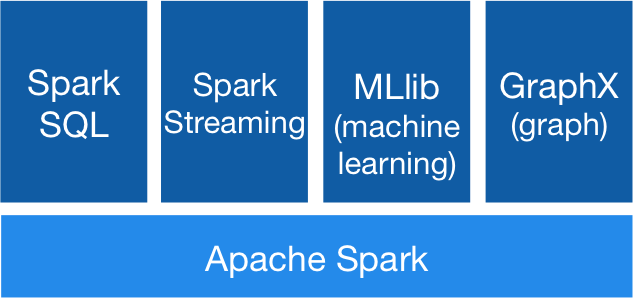
\includegraphics[width=0.8\textwidth]{spark-stack}
	\caption{Spark Stack}
\end{figure}


Spark optimizes for iterative computations, which allows users to load data to the cluster memory, and do repeated operation on these data many times, which makes it very suitable for machine learning\cite{meng2016mllib}.

\section{Comparison between MapReduce and Spark}
The simplicity of MapReduce is attractive for developers but this framework has some limitations. MapReduce is designed to batch jobs which makes it not good at iterative computations that need to run the same mapper and reducer multiple times, with output from the reducer as input to mapper of the next stage (like machine learning application)\cite{shi2015clash}. Let's use Hadoop MapReduce, a widely used implementation to describes this shortcomings. As shown in Figure~\ref{fg:hadoop}, while Hadoop MapReduce is processing computing, it need to store intermediate data into HDFS, which causes extensive data movement and duplication across the network and file system. As a result, HDFS I/O is often the bottleneck of this system.

\begin{figure}[h]
	\centering
	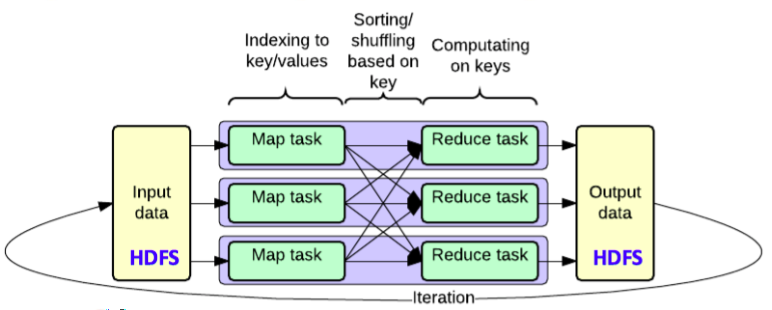
\includegraphics[width=0.9\textwidth]{hadoopcycle}
	\caption{Data cycle in Hadoop MapReduce}
	\label{fg:hadoop}
\end{figure}

From the above description, MapReduce do not have efficient data sharing method. Spark solve this problem using in-memory data processing and sharing\cite{apache_spark}. As shown in Figure~\ref{fg:spark}, Spark is based on the in-memory framework. While computing, those intermediate data is temporarily stored in memory, which greatly speed up the execution. Especially for those applications that needs iterations.

\begin{figure}[h]
	\centering
	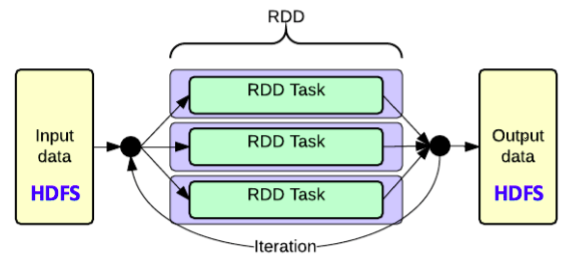
\includegraphics[width=0.8\textwidth]{sparkcycle}
	\caption{Data cycle in Apache Spark}
	\label{fg:spark}
\end{figure}

The result in contest also prove this theory. In the Daytona GraySort contest for 2014, Apache Spark wins the first price\cite{3_xin_2014}. Results can be find in table~\ref{tb:hadoop_vs_spark}. Spark sorted the same data 3X faster using 10X fewer machines.
\begin{table}[h]
	\centering
	\resizebox{\textwidth}{!}{%
		\begin{tabular}{|l|c|c|c|}
			\hline
			& \textbf{Hadoop World Record} & \textbf{Spark 100 TB} & \textbf{Spark 1 PB} \\ \hline
			\textbf{Data Size} & 102.5 TB & 100 TB & 1000 TB \\ \hline
			\textbf{Elapsed Time} & 72 mins & 23 mins & 234 mins \\ \hline
			\textbf{\# Nodes} & 2100 & 206 & 190 \\ \hline
			\textbf{\# Coes} & 50400 & 6592 & 6080 \\ \hline
			\textbf{\# Reducers} & 10,000 & 29,000 & 250,000 \\ \hline
			\textbf{Rate} & 1.42 TB/min & 4.27 TB/min & 4.27 TB/min \\ \hline
			\textbf{Rate / node} & 0.67 GB/min & 20.7 GB/min & 22.5 GB/min \\ \hline
			\textbf{Sort Benchmark Daytona Rules} & Yes & Yes & No \\ \hline
			\textbf{Environment} & dedicated data center & EC2 (i2.8xlarge) & EC2 (i2.8xlarge) \\ \hline
		\end{tabular}%
	}
	\caption{Spark TeraSort vs MapReduce\cite{3_xin_2014}}
	\label{tb:hadoop_vs_spark}
\end{table}


\section{Core Data Structure in Spark}

Resilient distributed datasets and dataframe are the basic data structure used in Spark to handle data.\\

\subsection{Resilient Distributed Datasets}

Resilient distributed datasets, or RDD, designed based on Matei\cite{zaharia2012resilient}, is one of the core technology in Spark frame. RDD can be regard as a table in database, which can hold any type of data. Spark save data to different partitions RDD.\\


Every RDD can contain many partitions, a partition is a part of dataset. RDD can rely on each other. The case that each partition of the parent RDD is used by at most one partition of the child RDD is called narrow dependency, data shuffling is unnecessary in this type of operation; while multiple child partitions may depend on one parent partition is called wide dependencies, this type of operations involves data shuffling.
\begin{figure}[h]
	\centering
	\subfigure[Narrow Dependency]{
		\centering
		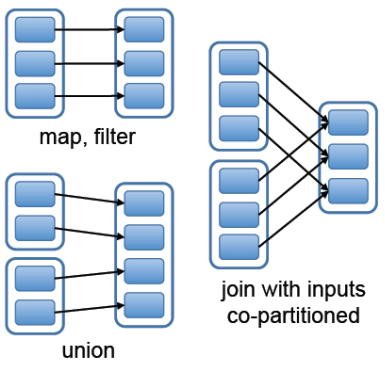
\includegraphics[width=.6\linewidth]{narrowdependencies}
	}
	\subfigure[Wide Denpendency]{
		\centering
		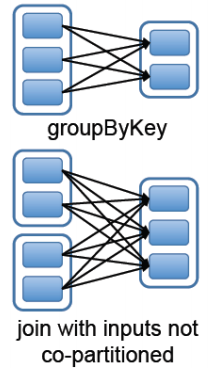
\includegraphics[width=.3\linewidth]{widedependences}
	}
	\caption{Two types of Spark Dependency\cite[p.~8]{zaharia2012resilient}}
\end{figure}

There are two reasons that why Spark make narrow dependencies out of wide one\cite[Chapter~5]{zaharia2012resilient},
\begin{enumerate}
	\item Narrow allow for pipelined execution on one cluster node, while wide dependencies must wait for all the parent partitions available.
	\item Fault recover is much easier for narrow dependencies, as it just need to re-compute the lost partitions, and this operation can be done in different nodes. On the other hand, wide dependencies involves many parent partitions.
\end{enumerate}

RDDs are immutable, the returns of every operation on RDD is a new RDD. RDD support two types of operations,

\begin{enumerate}
	\item Transformation\cite[Section~2.2]{zaharia2012resilient}: each transformation takes (one or more) RDDs, and outputs the transformed RDD (another RDD) by applying some function to the contents (e.g., map, filter, groupBy). All transformations in Spark are lazy, only computed when an action requires a result to be returned to the driver program.
	\item Action\cite[Section~2.3]{zaharia2012resilient}: Return a value to the driver program after running a computation on the dataset (e.g., reduce, reduceByKey, etc.). An action is used to either save result to some location (HDFS) or to display it via the driver program.
\end{enumerate}

To solve the problems about fault tolerance, RDD support two type of operation

\begin{enumerate}
	\item An automatic way, the RDDs log lineage (the sequence of transformations used to produce the current RDD) information\cite[Section~2.5]{zaharia2012resilient}. And when data lost happened, spark would recursively go back to the very root, or the previous checkpoint, and then re-compute the lost data.
	\item User can manually set checkpoint, at which Spark would truncated lineages and store data in reliably location, like HDFS\cite[Section~5.3]{zaharia2012resilient}.
\end{enumerate}

\subsection{Spark SQL and DataFrame}
Spark SQL was first released in May 2014. The Goal of Spark SQL is to provide an efficient, extensive and programmer-friendly API within Spark programs (on native RDDs)\cite{armbrust2015spark}.\\ 

Spark SQL runs on top of Spark. Its structure is shown in figure~\ref{fg:spark_structure}. Spark SQL provide a data structure called DataFrame (Which was first released in Spark 1.3.0 on Mar. 13, 2015. \footnote{\url{http://spark.apache.org/releases/spark-release-1-3-0.html}}). This API is similar to the data frame concept in R\footnote{The R Project, \url{https://www.r-project.org/}} and python\footnote{Python Data Analysis Library \url{http://pandas.pydata.org/}}.\\

\begin{figure}[h]
	\centering
	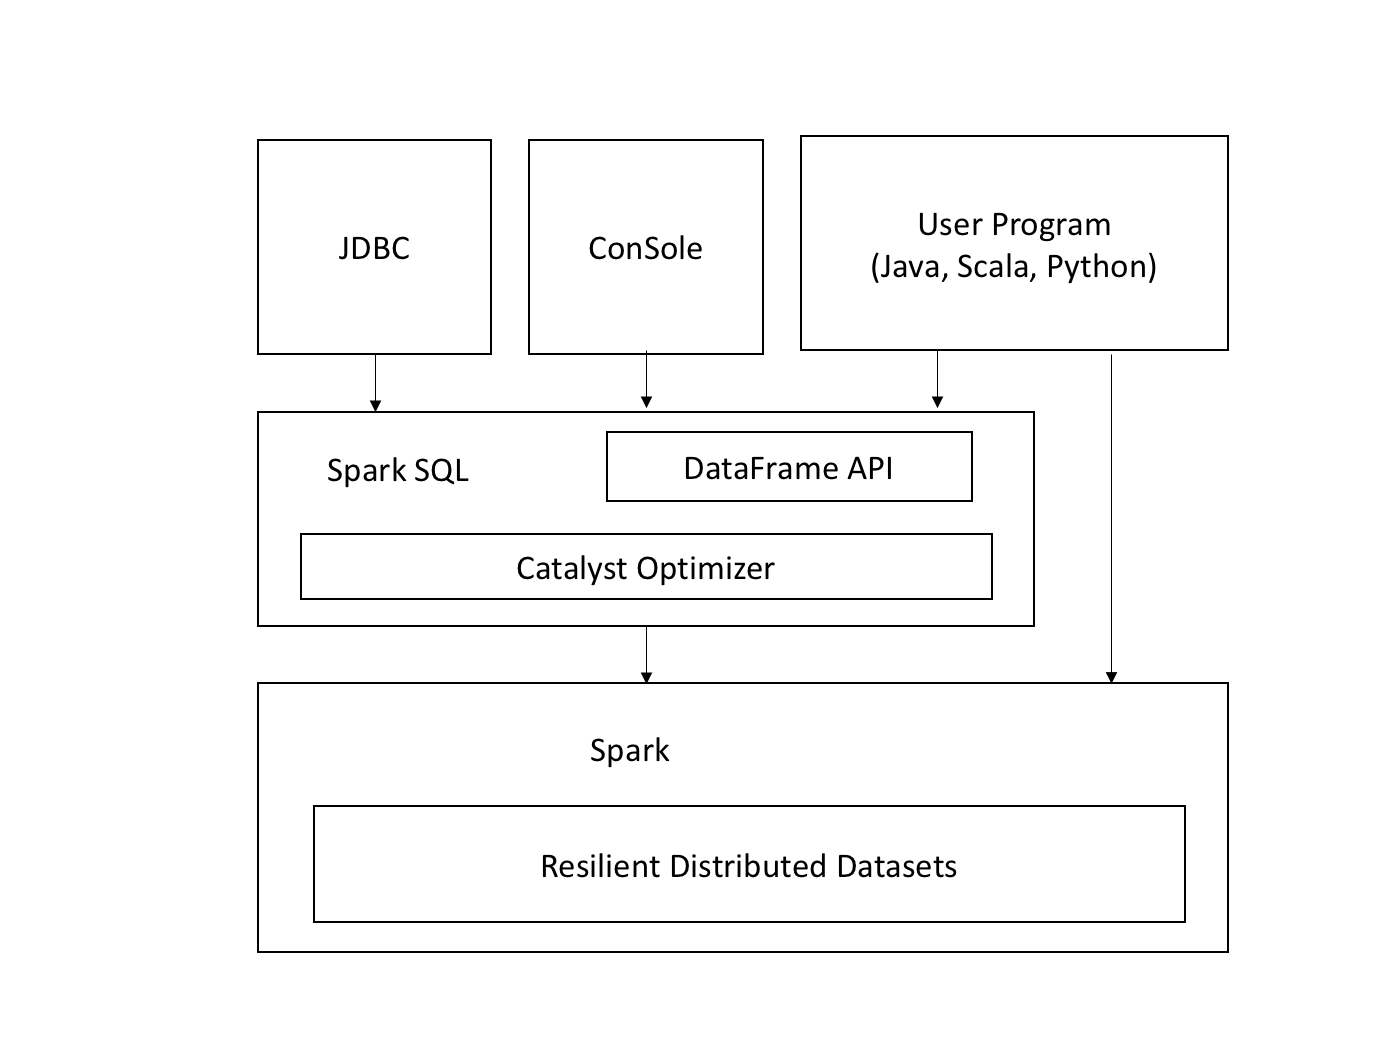
\includegraphics[width=0.8\textwidth]{DistributedSystem/Interface}
	\caption{Interfaces to Spark SQL, and interaction with Spark\cite{armbrust2015spark}.}
	\label{fg:spark_structure}
\end{figure}


Similar to RDDs, Spark DataFrames are also lazy, ``in that each DataFrame object represents a \textit{logical plan} to compute a dataset, but no execution occurs until the user calls a special '\textit{output operation}' such as \textit{save}.''\cite{armbrust2015spark}


\section{Spark Machine Learning Library (MLlib \& ML)}
Apart from the above benefits, MLlib is another reason that why we choose spark. MLlib is the extensible machine learning  library of Spark, which composes of general learning algorithm and utilities, includes classification, regression, clustering, collaborative filtering, dimension reduction and tuning section\cite{meng2016mllib}.\\


As native supported by Apache Spark, MLlib has the following benefits\cite{meng2016mllib}: First, since Apache Spark is designed for iterative applications, MLlib directly gains benefits through the improvements of Spark's low-level components. Second, the widely accepted by open-source community of Spark has also led to rapid growth and adoption of MLlib. Third, MLlib has great performances advantages over Mahout, another popular distributed machine learning library. Experiments in \cite{1_li_jiang_zhang_boesch_xiao_2015} shows that MLlib is about 7--9 times faster than Mahout in FP-growth mining problem.\\


From version 1.2, Spark MLlib was divided into two libraries, MlLib and ML\footnote{Spark Release Note 1.2.0 \url{http://spark.apache.org/releases/spark-release-1-2-0.html}}. MlLib contains the original API built on top of RDDs, while ML provides higher-level API built on top of Spark DataFrames for constructing ML pipelines.\\


Ml is more recommended by the official document, but MlLib is still being supported. This dissertation was based on both MlLib, and ML.


\section{Summary}
Apache Spark is an open source framework optimized for iterative programs, like machine learning. That is why this study chooses Spark instead of MapReduce.\\


The core technology of Spark is RDD, an immutable distributed data structure, which support two types of operation, transformation and action. RDD can be saved any type of storage, but usually is cached in memory.\\


Spark SQL offers DataFrame API, which is also lazy but more similar to data frame concept in R and Python. Compares to RDD, Spark DataFrame offers much more programmer-friendly API.\\


This study chooses MLlib because of its ease of use and tight integration with Spark.


 % Introduction to Cloud Computing

\chapter{Data Mining Methods}
\label{ch:mining}

This chapter introduces the data transformation method used in this dissertation.
\section{Remove invalid or missing data}
As a real-world applications of data mining, there are some invalid or missing data in the original data collection. This system should automatically remove invalid data from the raw data and replace missing values with rational information. The rule to handle data is as follows,

\clearpage
\begin{itemize}
	\item Data on holiday. One example is in figure~\ref{fg:invalid_data}, Jan 1, 2016 is New Year Day, and Dec 25, 2015 is Christmas day. There are no transactions on these two days, but in Yahoo Finance, holidays like there are still listed there. Information about Hong Kong holidays are collected from http://www.timeanddate.com/, and after downloading data from Yahoo Finance, the system would automatically remove these holiday transaction data.
	\begin{figure}[h]
		\centering
		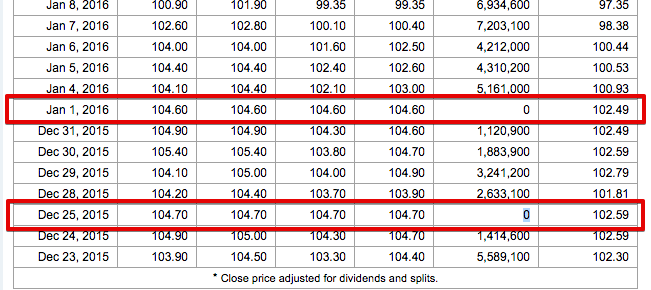
\includegraphics[width=0.9\textwidth]{invalid-data}
		\caption{Example for invalid data}
		\label{fg:invalid_data}
	\end{figure}
\end{itemize} % Introduction to Data mining method used in this thesis

\chapter{System Design and Evaluation Method}
\label{ch:system}

The objective of this dissertation is to build an automatic system which can download raw data, do transformation, train model, and give prediction result. This system is based on Python, a Friendly power programming language. “Quandl”, “TA-Lib”, “SciPy”, “pySpark”, “SciPy-learner” are used for data collecting, mining analysis and handling times series data structure. The whole process can be found in figure~\ref{fg:system_model}.
\begin{figure}[h]
	\centering
	\includegraphics[width=0.6\textwidth]{Model/FlowChart}
	\caption{Flow Chart of the whole system}
	\label{fg:system_model}
\end{figure}

After collected all raw data, system would split it into two parts, training and testing (details about collected data is introduced in Chapter\ref{ch:market}). To make an convincing experiment, \emph{the date of all testing data is behind that of training data}, so that the system would have no knowledge of the testing data. Let's talk about the details of data processing and model training process next.\\


\section{Data Processing}
The data processing part include data normalization and PCA. Feature vectors of testing and training data, labels of training data should be normalized, technique details are introduced in Chapter~\ref{ch:mining}.\\


Feature vectors transform process are,
\begin{enumerate}
	\item Train a data normalizer (Min Max Normalization) and translate training features into normalized data.
	\item Train a PCA transformer using step 1's output, and transform those data.
	\item Train a second data normalizer (also Min Max Normalization) and translate step 2's output into processed data.
	\item Use the same transformer in step 1-3 to transform testing features step by step.
\end{enumerate}

The label data process only handles training data, there are two types of transform method based on the model used in next step,
\begin{itemize}
	\item If training model is single learning algorithm, i.e., the model are used to predict the stock price directly. Then the label is normalized based on the high and low price of last five days,
	\begin{equation}
		label'=\frac{label*2-(high + low)}{high - low}
	\end{equation}
	\item If training model is the combine of two learning algorithm, i.e., one is used to predict change direction, the other is to forecast amount. The trend label is transformed with,
	\begin{equation}
	trend=\begin{cases}
	1 & \text{ if } price_{tomorrow} > price_{today} \\ 
	0 & \text{ if } otherwise
	\end{cases}
	\end{equation}
	The amount label is calculated by,
	\begin{equation}
	amount=\left | price_{tomorrow} - price_{today} \right |
	\end{equation}
	and after the above calculation, the amount value will be normalized using standard normalization algorithm. 
\end{itemize}

After the above process, data is transformed and can be used for model training.


\section{Training and Predict}
As described before, there are two learning method used in this dissertation. 
\begin{itemize}
	\item Using one single algorithm to predict the stock price directly. Such algorithms include Linear Regression, Random Forest and ANN
	\item A combination of two learning method, using one algorithm to predict change direction (Logistic Regression, Random Forest and SVM), another to forecast amount (Linear Regression, Random, Forest and ANN). The two method works separately, and the predict result is the combination of both model.
\end{itemize}

On each iteration, system would randomly subsample the origin training dataset to get a different training set (a.k.a. bootstrapping). If the training algorithm does not support re-training (like Random Forest and SVM in pyspark.mllib), then the best model would be picked. Otherwise, just re-train the former model.\\


After training, the system would get a model then uses it to predict from testing dataset.



\section{Model Evaluation}
Compare forecasting performance of different learning method is one of the most important task of prediction study. This section introduces the criteria used in this dissertation.\\


let $ \hat{p} $ be the predicted variable, $ p $ be the actual stock price, $ \epsilon = \hat{p} - p $ be the forecast error, and $ N $ be the number of total testing sample number. Popular evaluation measures used in this study includes\cite{poon2005practical},
\begin{itemize}
	\item \textit{Mean Error} (ME)
	\begin{equation}
	ME=\frac{1}{N} \sum_{i=1}^{N}\epsilon_i=\frac{1}{N} \sum_{i=1}^{N} (\hat{p}_i - p_i)
	\end{equation}
	
	\item \textit{Mean Square Error} (MSE)
	\begin{equation}
	MSE = \frac{1}{N} \sum_{i=1}^{N}\epsilon_i^2=\frac{1}{N} \sum_{i=1}^{N} (\hat{p}_i - p_i)^2
	\end{equation}
	
	\item \textit{Root Mean Square Error} (RMSE)
	\begin{equation}
	RMSE = \sqrt{\frac{1}{N} \sum_{i=1}^{N}\epsilon_i^2}=\sqrt{\frac{1}{N} \sum_{i=1}^{N} (\hat{p}_i - p_i)^2}
	\end{equation}
	
	\item \textit{Mean Absolute Error} (MAE)
	\begin{equation}
	MAE=\frac{1}{N} \sum_{i=1}^{N} \lvert \epsilon_i \rvert =\frac{1}{N} \sum_{i=1}^{N} \lvert \hat{p}_i - p_i \rvert
	\end{equation}
	
	\item \textit{Mean Absolute Percent Error} (MAPE)
	\begin{equation}
	MAPE=\frac{1}{N} \sum_{i=1}^{N} \frac{\lvert \epsilon_i \rvert}{p_i} =\frac{1}{N} \sum_{i=1}^{N} \frac{\lvert \hat{p}_i - p_i \rvert}{p_i}
	\end{equation}
	
	\item \textit{Heteroscedasticity-adjust Mean Square Error} (HMSE)
	\begin{equation}
	HMSE=\frac{1}{N} \sum_{i=1}^{N}[\frac{p_i}{\hat{p}_i}- 1]^2
	\end{equation}
\end{itemize}
The first four measurements is scaled by predicted volatility, which are suitable to compare the prediction of same stock during equal period. The later two can be used to compare every method as they represent percentage errors.\\


In addition to knowing the amount of changes measurement, the direction of prices is also very important. Here, corrected direction change (CDC)\cite{naeini2010stock} are used
\begin{equation}
CDC = \frac{\text{Number of Corrected Forecast Trend}}{N}
\end{equation}
A completely random prediction should have $ 50\% $ CDC, so for a reliable forecast, this value should be greater than $ 50\% $\\


This is no measurement that are perfect enough to compare all learning algorithms, all criteria would be considered as a whole. Besides, as there are some randomness in the training method, all the result would be tested 3 times and get the average. % Software model

\chapter{Data Preproesssing}

Lorem ipsum dolor sit amet, consectetur adipiscing elit. Vivamus at pulvinar nisi. Phasellus hendrerit, diam placerat interdum iaculis, mauris justo cursus risus, in viverra purus eros at ligula. Ut metus justo, consequat a tristique posuere, laoreet nec nibh. Etiam et scelerisque mauris. Phasellus vel massa magna. Ut non neque id tortor pharetra bibendum vitae sit amet nisi. Duis nec quam quam, sed euismod justo. Pellentesque eu tellus vitae ante tempus malesuada. Nunc accumsan, quam in congue consequat, lectus lectus dapibus erat, id aliquet urna neque at massa. Nulla facilisi. Morbi ullamcorper eleifend posuere. Donec libero leo, faucibus nec bibendum at, mattis et urna. Proin consectetur, nunc ut imperdiet lobortis, magna neque tincidunt lectus, id iaculis nisi justo id nibh. Pellentesque vel sem in erat vulputate faucibus molestie ut lorem.

\section{A Section}

Quisque tristique urna in lorem laoreet at laoreet quam congue. Donec dolor turpis, blandit non imperdiet aliquet, blandit et felis. In lorem nisi, pretium sit amet vestibulum sed, tempus et sem. Proin non ante turpis. Nulla imperdiet fringilla convallis. Vivamus vel bibendum nisl. Pellentesque justo lectus, molestie vel luctus sed, lobortis in libero. Nulla facilisi. Aliquam erat volutpat. Suspendisse vitae nunc nunc. Sed aliquet est suscipit sapien rhoncus non adipiscing nibh consequat. Aliquam metus urna, faucibus eu vulputate non, luctus eu justo.

\subsection{A Subsection}

Donec urna leo, vulputate vitae porta eu, vehicula blandit libero. Phasellus eget massa et leo condimentum mollis. Nullam molestie, justo at pellentesque vulputate, sapien velit ornare diam, nec gravida lacus augue non diam. Integer mattis lacus id libero ultrices sit amet mollis neque molestie. Integer ut leo eget mi volutpat congue. Vivamus sodales, turpis id venenatis placerat, tellus purus adipiscing magna, eu aliquam nibh dolor id nibh. Pellentesque habitant morbi tristique senectus et netus et malesuada fames ac turpis egestas. Sed cursus convallis quam nec vehicula. Sed vulputate neque eget odio fringilla ac sodales urna feugiat.

\section{Another Section}

Phasellus nisi quam, volutpat non ullamcorper eget, congue fringilla leo. Cras et erat et nibh placerat commodo id ornare est. Nulla facilisi. Aenean pulvinar scelerisque eros eget interdum. Nunc pulvinar magna ut felis varius in hendrerit dolor accumsan. Nunc pellentesque magna quis magna bibendum non laoreet erat tincidunt. Nulla facilisi.

Duis eget massa sem, gravida interdum ipsum. Nulla nunc nisl, hendrerit sit amet commodo vel, varius id tellus. Lorem ipsum dolor sit amet, consectetur adipiscing elit. Nunc ac dolor est. Suspendisse ultrices tincidunt metus eget accumsan. Nullam facilisis, justo vitae convallis sollicitudin, eros augue malesuada metus, nec sagittis diam nibh ut sapien. Duis blandit lectus vitae lorem aliquam nec euismod nisi volutpat. Vestibulum ornare dictum tortor, at faucibus justo tempor non. Nulla facilisi. Cras non massa nunc, eget euismod purus. Nunc metus ipsum, euismod a consectetur vel, hendrerit nec nunc. % How to processing the data

\chapter{Details of System}
\label{ch:modelTrainingProcess}

This chapters shows the details of whole system, including parameters of all training and transforming algorithm, and processing of each part.

\section{Detail Parameters}
Details of the parameters can be found in Table~\ref{tb:parameters}

\begin{table}[h]
	\centering
	\begin{tabular}{|l|l|l|}
		\hline
		\multicolumn{1}{|c|}{\textbf{Algorithm}} & \multicolumn{1}{c|}{\textbf{Parameters}} & \multicolumn{1}{c|}{\textbf{Optimize Method}} \\ \hline
		\textbf{\begin{tabular}[c]{@{}l@{}}Random Forest\\ (Classifier \& Regressor)\end{tabular}} & \begin{tabular}[c]{@{}l@{}}Trees Number: 40\\ Max Depth: 20\end{tabular} & NA \\ \hline
		\textbf{SVM} & \begin{tabular}[c]{@{}l@{}}Iterations: 100000\\ Learning rate: 0.001\end{tabular} & SGD \\ \hline
		\textbf{Logistic Regression} & \begin{tabular}[c]{@{}l@{}}Iterations: 100000\\ Learning rate: 0.001\end{tabular} & SGD \\ \hline
		\textbf{Linear Regression} & \begin{tabular}[c]{@{}l@{}}Iterations: 100000\\ Learning rate: 0.001\end{tabular} & SGD \\ \hline
		\textbf{ANN} & \begin{tabular}[c]{@{}l@{}}Iterations: 15\\ Learning rate: 0.0001\end{tabular} & BGD \\ \hline
	\end{tabular}
	\caption{Parameters of Every learning method}
	\label{tb:parameters}
\end{table}


For the normalization method, the range of min-max normalizer is $ [-1, 1] $.\\

The PCA transformer follows the default configuration in sklearn.\\

The neural network is a four-layer (two hidden layer) model. A two-layer model is just same as linear regression. The reason for choosing 2 hidden layers is that "can represent an arbitrary decision boundary to arbitrary accuracy with rational activation functions and can approximate any smooth mapping to any accuracy"\cite[p.~128]{heaton2008introduction}.\\


To determine the number of neurons use in the hidden layers, Jeff Heaton also wrote in \cite[p.~129]{heaton2008introduction} that "The number of hidden neurons should be between the size of the input layer and the size of the output layer". So, in this study, the nodes number of the first hidden layer is $ \frac{2}{3} $ of that of the input layer, and that of the second is $ \frac{1}{3} $ of that of the input layer.

\section{Data Mining Processing}
The data mining process in this system include data preprocessing, data normalization, PCA transformation, model training and price prediction. The technique details about data process are introduced in Chapter~\ref{ch:mining}. Data clean process just follows the rules introduced in section~\ref{sec:dataClean}, let's start with the transformation process.

\subsubsection{Data Transformation (Normalization and PCA)}

Feature vectors transform process are,
\begin{enumerate}
	\item Train a data normalizer (Min Max Normalization) and translate training features into normalized data.
	\item Train a PCA transformer using step 1's output, and transform those data.
	\item Train a second data normalizer (also Min Max Normalization) and translate step 2's output into processed data.
	\item Use the same transformer in step 1-3 to transform testing features step by step.
\end{enumerate}

The label data process only handles training data, there are two types of transform method based on the model used in next step,
\begin{itemize}
	\item If training model is single learning algorithm, i.e., the model are used to predict the stock price directly. Then the label is normalized based on the high and low price of last five days,
	\begin{equation}
	label'=\frac{label*2-(high + low)}{high - low}
	\end{equation}
	\item If training model is the combine of two learning algorithm, i.e., one is used to predict change direction, the other is to forecast amount. The trend label is transformed with,
	\begin{equation}
	trend=\begin{cases}
	1 & \text{ if } price_{tomorrow} > price_{today} \\ 
	0 & \text{ if } otherwise
	\end{cases}
	\end{equation}
	The amount label is calculated by,
	\begin{equation}
	amount=\left | price_{tomorrow} - price_{today} \right |
	\end{equation}
	and after the above calculation, the amount value will be normalized using standard normalization algorithm. 
\end{itemize}

After the above process, data is transformed and can be used for model training.

\subsection{Model Training and Predicting process}
As described before, there are two types of combination of learning methods used in this dissertation. 
\begin{itemize}
	\item Using one single algorithm to predict the stock price directly. Such algorithms include Linear Regression, Random Forest and ANN
	\item A combination of two learning method, using one algorithm to predict change direction (Logistic Regression, Random Forest and SVM), another to forecast amount (Linear Regression, Random, Forest and ANN). The two method works separately, and the predict result is the combination of both model.
\end{itemize}
 % How to training the model

\chapter{Model Accuracy Results}
\label{ch:AccuracyResult}
In this chapter, all test result would be represented and discussed here. Most of those test results try to predict one year stock price. The addition result can be found in Appendix~


\section{Using 4 years historical data}

The test slot is from 2010-01-06 to 2015-01-06, the first four year data (from 2010-01-06 to 2014-01-05) are training dataset (986 transaction days), the remaining used to act as testing data (test size is 248).\\


The average stock price over this period is showed in table~\ref{tb:avg20142015} and the RMSE comparison is in figure~\ref{fg:4yearpredict1}, \ref{fg:4yearpredict2} and \ref{fg:4yearpredict3}. Average CDC info can be found in table~\ref{tb:averageCDC1}.\\


\begin{table}[h]
	\centering
	\begin{tabular}{|l|l|l|l|}
		\hline
		\textbf{Stock Symbol} & \textbf{Average Price(HKD)} & \textbf{Stock Symbol} & \textbf{Average Price (HKD)} \\ \hline
		\textbf{0001.HK}      & 94.9379262096775       & \textbf{0006.HK}      & 68.62278225806452      \\ \hline
		\textbf{0002.HK}      & 63.25927419354843      & \textbf{0007.HK}      & 1.316129032258065      \\ \hline
		\textbf{0003.HK}      & 19.05447125000001      & \textbf{0008.HK}      & 4.466854838709676      \\ \hline
		\textbf{0004.HK}      & 55.95322580645161      & \textbf{0009.HK}      & 0.6356521739130431     \\ \hline
		\textbf{0005.HK}      & 80.08870967741933      & \textbf{0010.HK}      & 39.71733870967743      \\ \hline
	\end{tabular}
	\caption{Average Stock Price (from 2014-01-06 to 2015-01-06)}
	\label{tb:avg20142015}
\end{table}

%\begin{figure}[h]
%	\centering
%	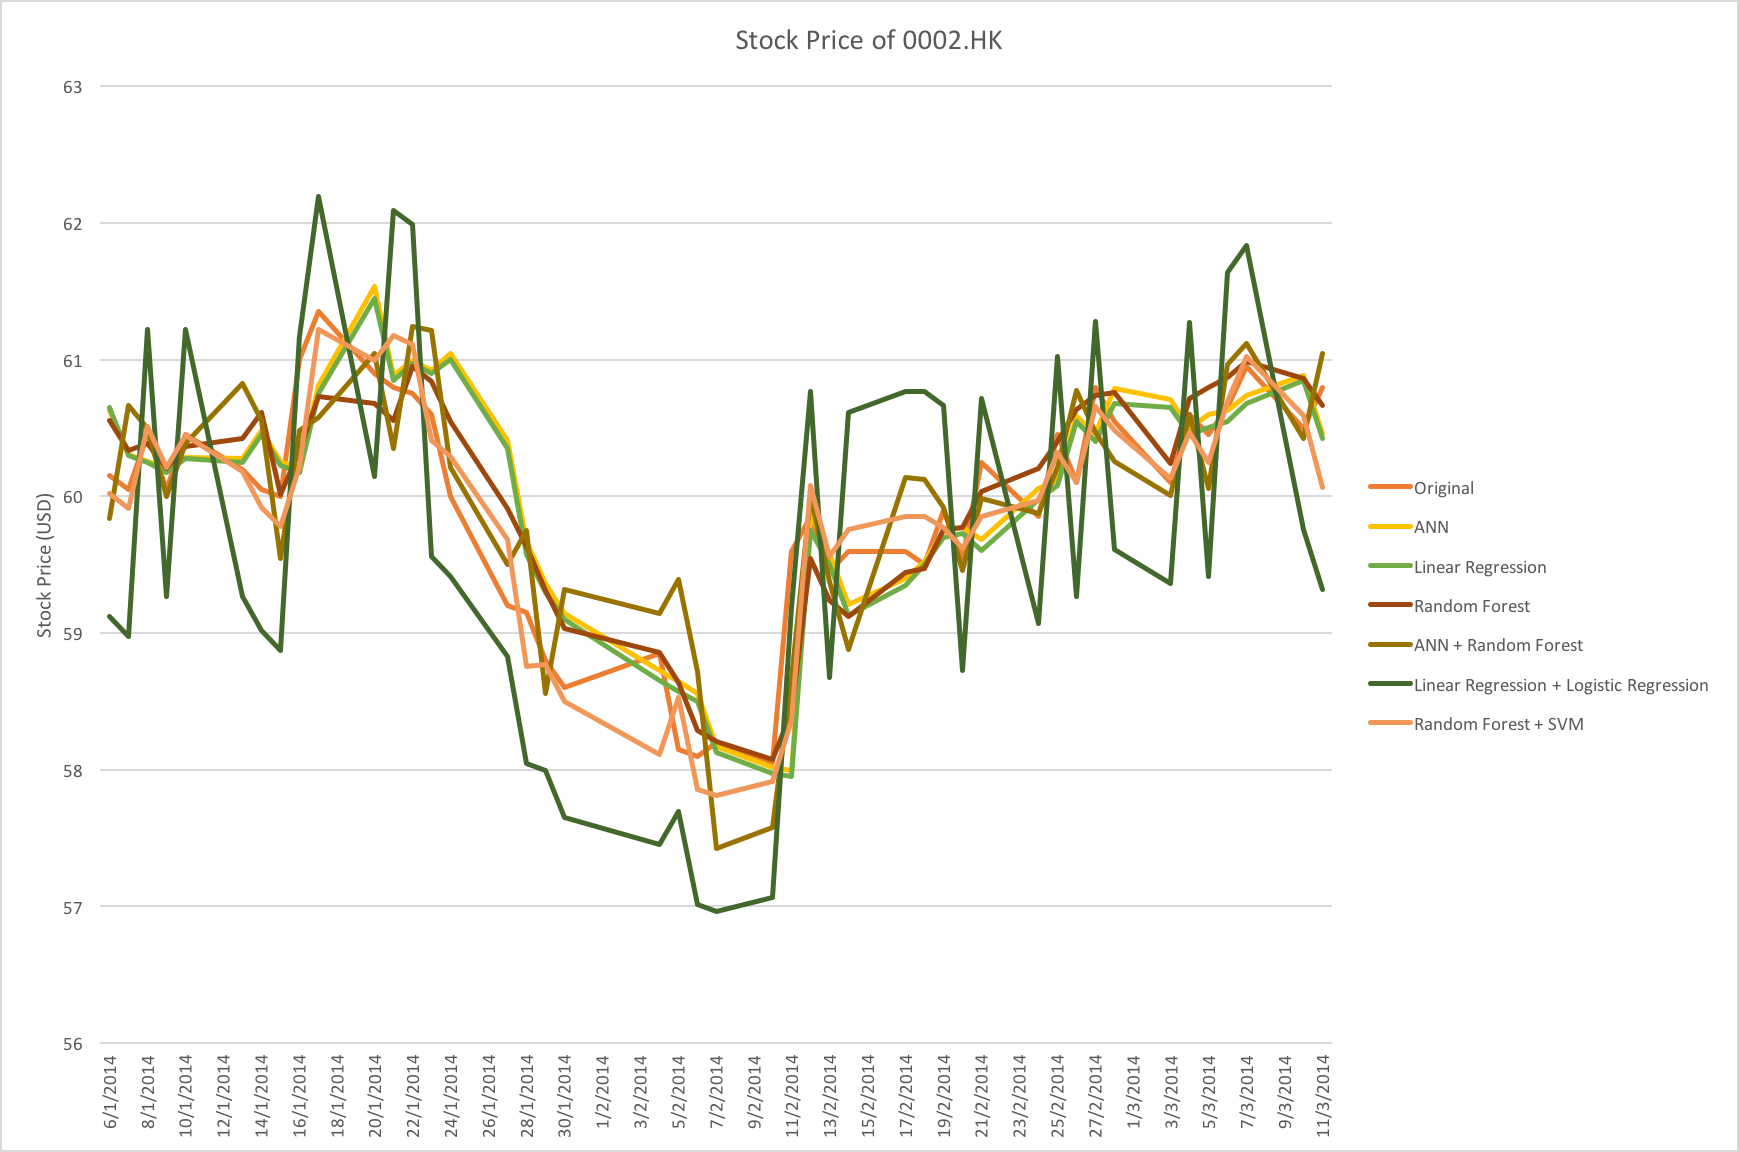
\includegraphics[width=.8\textwidth]{Result/20102015/0002}
%	\caption{Sample Predict prices of 0002.HK}
%\end{figure}

\begin{figure}[h]
	\centering
	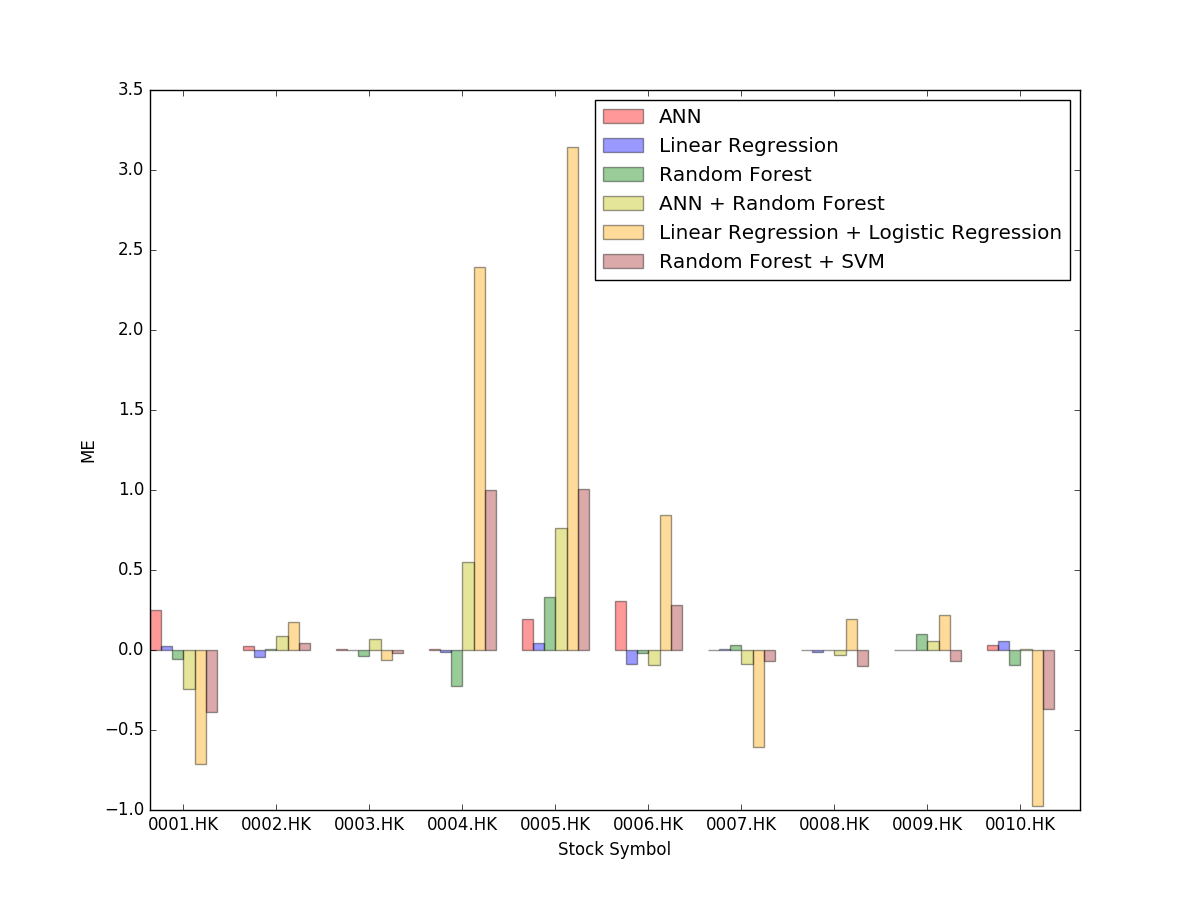
\includegraphics[width=.8\textwidth]{Result/20102015/ME}
	\caption{Testing result in time period 2014-01-07 to 2015-01-06}
	\label{fg:4yearpredict1}
\end{figure}

\begin{figure}[h]
	\centering
	\subfigure[RMSE]{
		\centering
		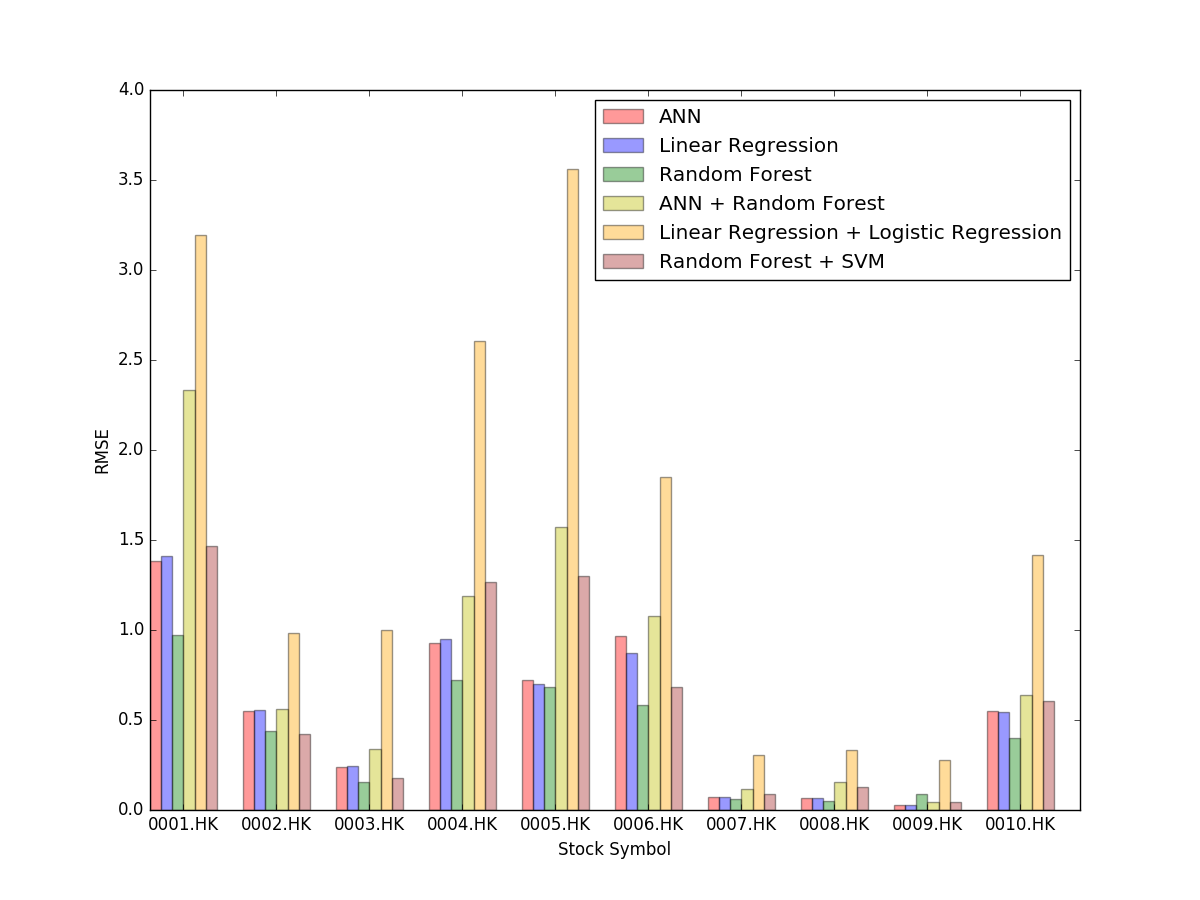
\includegraphics[width=.8\textwidth]{Result/20102015/RMSE}
	}
	\subfigure[CDC]{
		\centering
		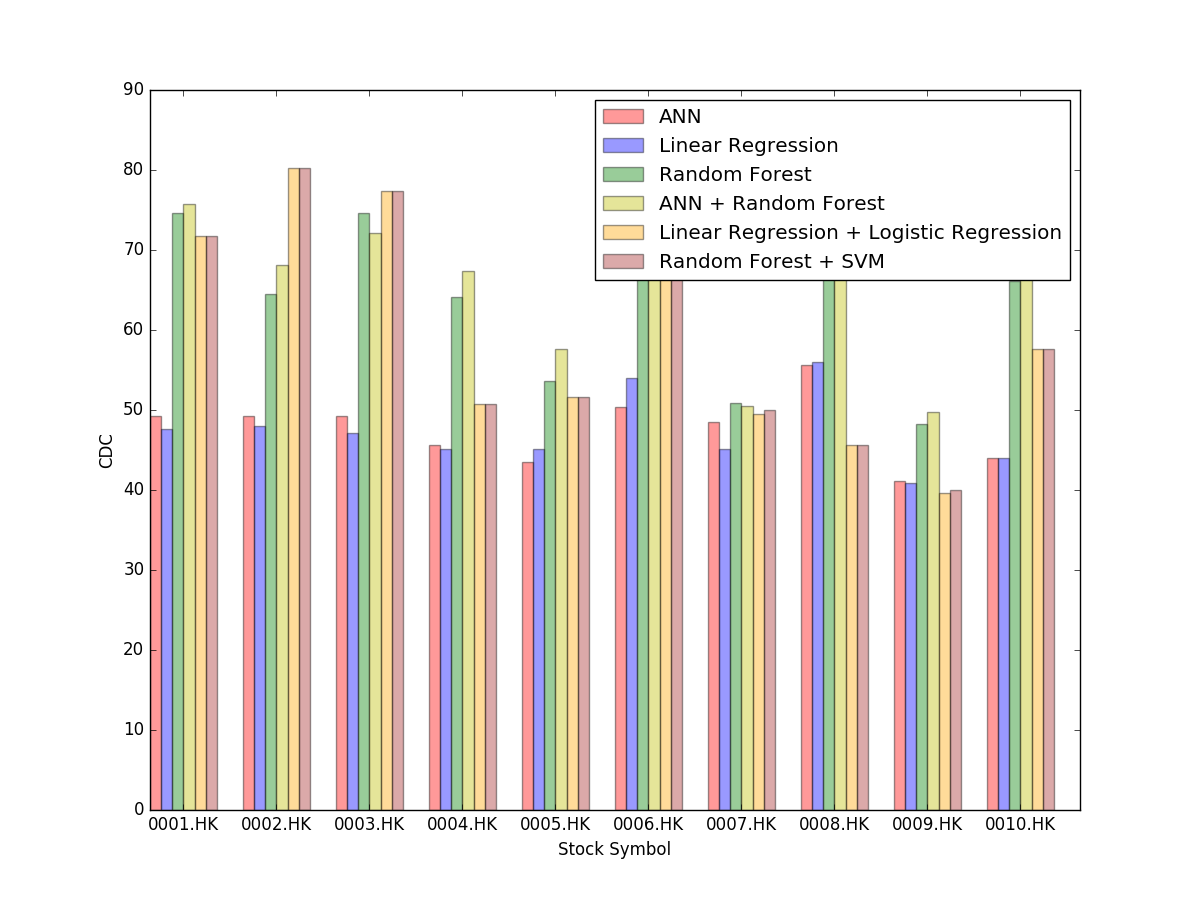
\includegraphics[width=.8\linewidth]{Result/20102015/CDC}
	}
	\caption{Testing result in time period 2014-01-07 to 2015-01-06 (continue)}
	\label{fg:4yearpredict2}
\end{figure}

\begin{figure}[h]
	\centering
	\subfigure[MAPE]{
		\centering
		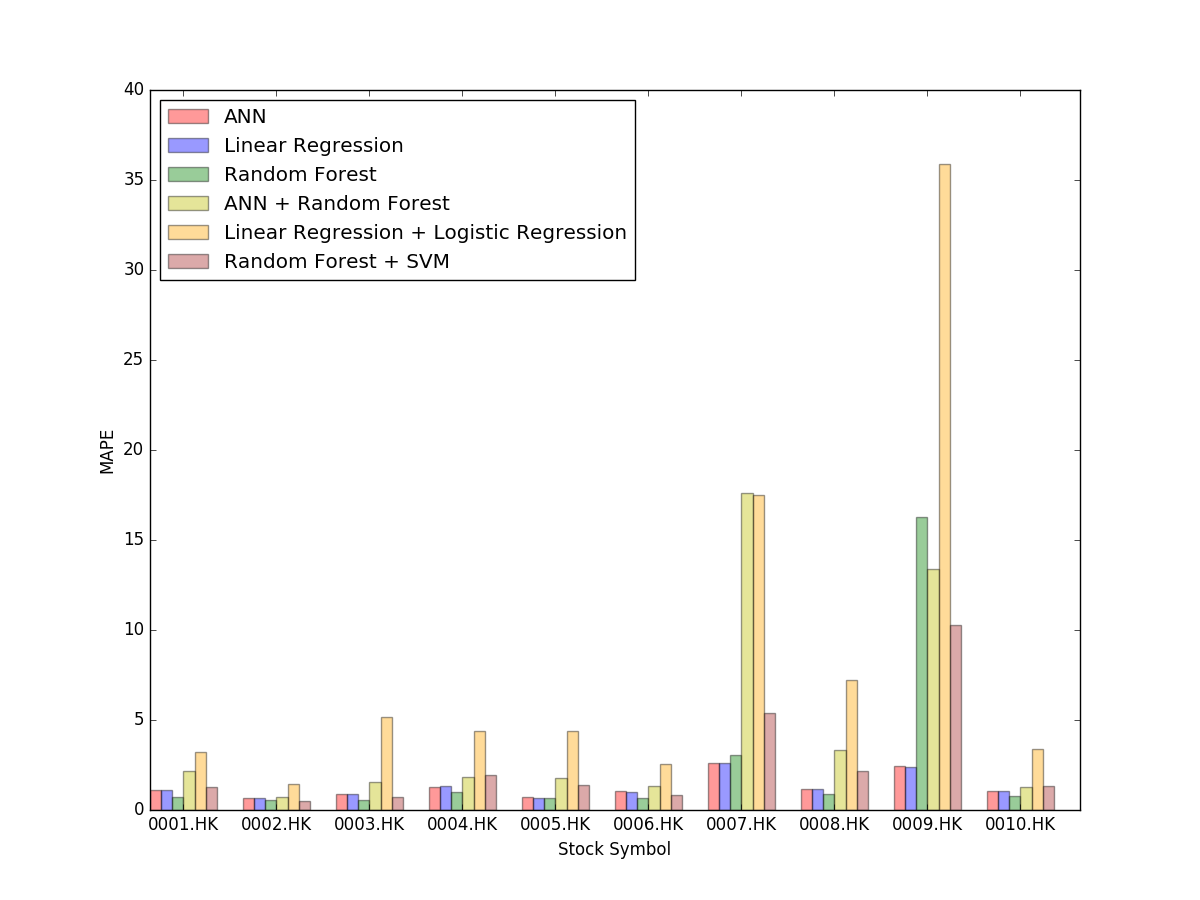
\includegraphics[width=.8\textwidth]{Result/20102015/MAPE}
	}
	\subfigure[HMSE]{
		\centering
		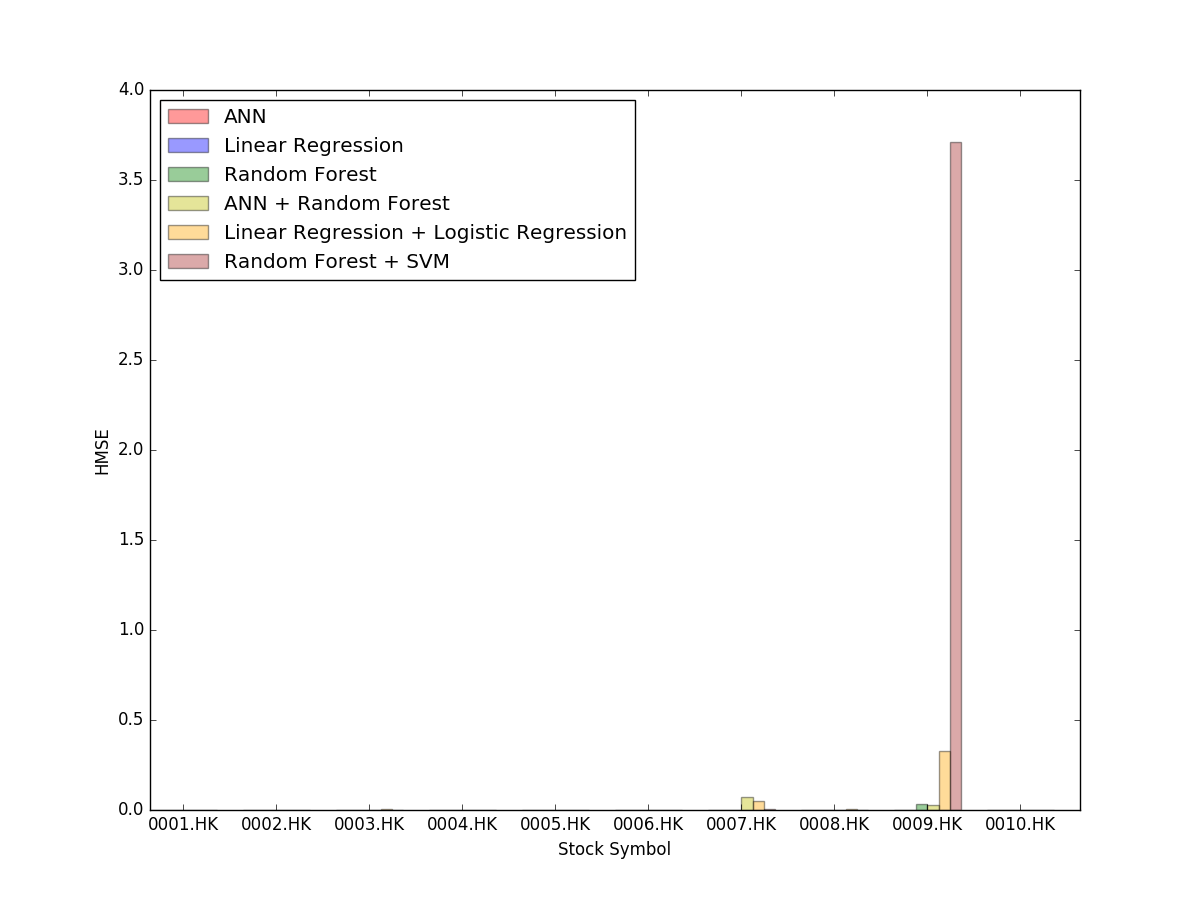
\includegraphics[width=.8\linewidth]{Result/20102015/HMSE}
	}
	\caption{Testing result in time period 2014-01-07 to 2015-01-06 (continue)}
	\label{fg:4yearpredict3}
\end{figure}

\begin{table}[h]
	\centering
	\begin{tabular}{|l|l|}
		\hline
		\textbf{Algorithm} & \textbf{Average CDC} \\ \hline
		\textbf{ANN} & 46.52\% \\ \hline
		\textbf{Linear Regression} & 46.61\% \\ \hline
		\textbf{Random Forest} & 63.20\% \\ \hline
		\textbf{\begin{tabular}[c]{@{}l@{}}Linear Regression \\ + Logistic Regression\end{tabular}} & 60.14\% \\ \hline
		\textbf{Random Forest + SVM} & 60.14\% \\ \hline
		\textbf{ANN + Random Forest} & 65.82\% \\ \hline
	\end{tabular}
	\caption{Average CDC in time period 2010-01-06 to 2015-01-06}
	\label{tb:averageCDC1}
\end{table}
\clearpage

The best learning algorithm under this circumstance is Random Forest, which has the second best CDC (In figure~\ref{fg:4yearpredict2}.b and table~\ref{tb:averageCDC1} the best algorithm is a combined method whose trend model is also based on Random Forest) and lowest error in amount prediction. And as both linear classifiers, the CDC result of Logistic Regression and SVM are almost same\\


For combination method, random forest algorithm is also the best model to predict stock price change amount. The performance of classifiers is also acceptable.


\section{Using 3 years historical data}

This time slot is from 2010-01-06 to 2014-01-06, the first three year data (from 2010-01-06 to 2013-01-06) are training dataset (train size is 743), the remaining used to act as testing data (test size is 244).\\


The average stock price over this period is showed in table~\ref{tb:avg20132014} and the RMSE comparison is in figure~\ref{fg:3yearpredict1}, \ref{fg:3yearpredict2} and \ref{fg:3yearpredict3}. Average CDC info can be found in table~\ref{tb:averageCDC2}.\\
\begin{table}[h]
	\centering
	\begin{tabular}{|l|l|l|l|}
		\hline
		\textbf{Stock Symbol} & \textbf{Average Price(HKD)} & \textbf{Stock Symbol} & \textbf{Average Price (HKD)} \\ \hline
		\textbf{0001.HK}      & 83.44622379       & \textbf{0006.HK}      & 68.2534274193548      \\ \hline
		\textbf{0002.HK}      & 64.5012096774194     & \textbf{0007.HK}      & 1.31673267326733      \\ \hline
		\textbf{0003.HK}      & 22.1624665322581      & \textbf{0008.HK}      & 3.55899193548387      \\ \hline
		\textbf{0004.HK}      & 66.6220647773279      & \textbf{0009.HK}      & 0.752991071428572     \\ \hline
		\textbf{0005.HK}      & 84.7485887096774      & \textbf{0010.HK}      & 42.6689516129032      \\ \hline
	\end{tabular}
	\caption{Average Stock Price (from 2013-01-06 to 2014-01-06)}
	\label{tb:avg20132014}
\end{table}

\begin{figure}[h]
	\centering
	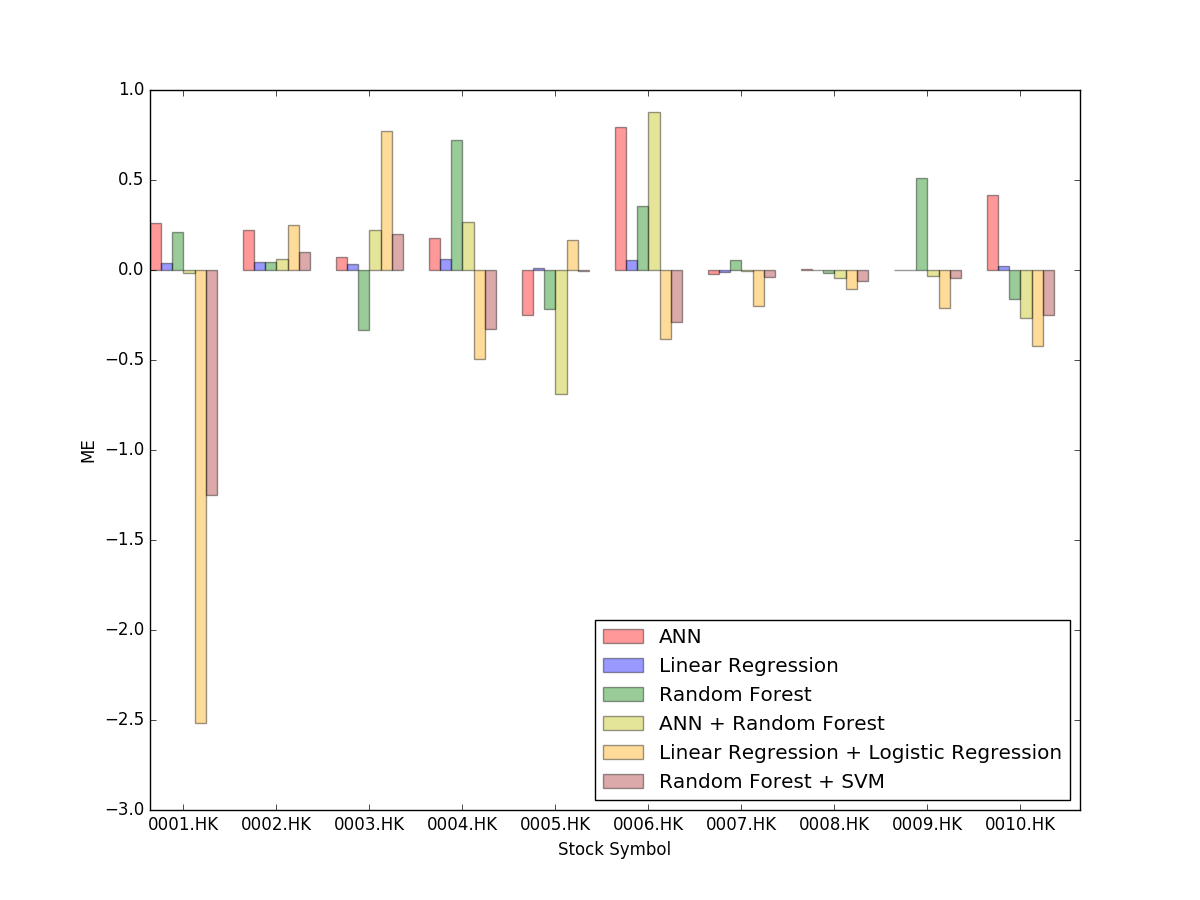
\includegraphics[width=.8\textwidth]{Result/3120102014/ME}
	\caption{Testing result in time period 2013-01-07 to 2014-01-06}
	\label{fg:3yearpredict1}
\end{figure}

\begin{figure}[h]
	\centering
	\subfigure[RMSE]{
		\centering
		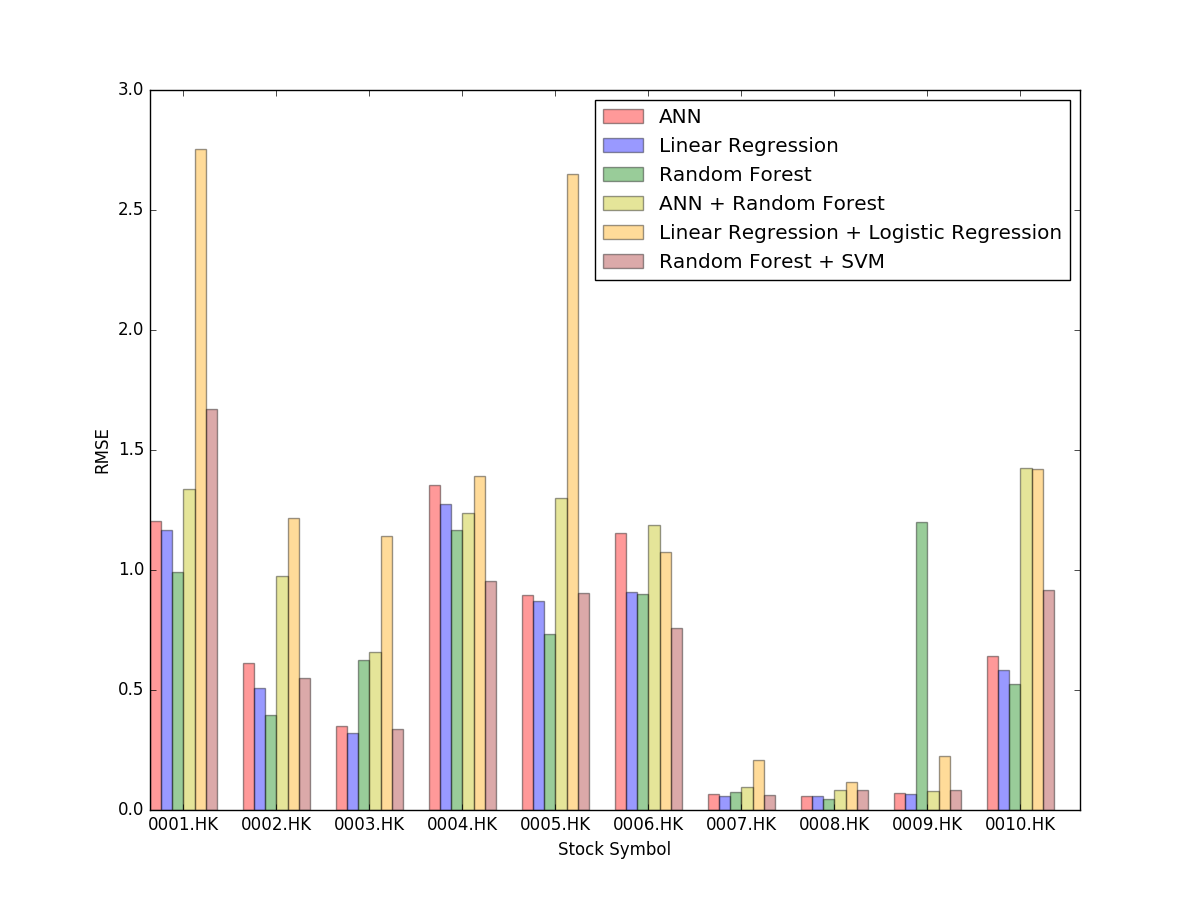
\includegraphics[width=.8\textwidth]{Result/3120102014/RMSE}
	}
	\subfigure[CDC]{
		\centering
		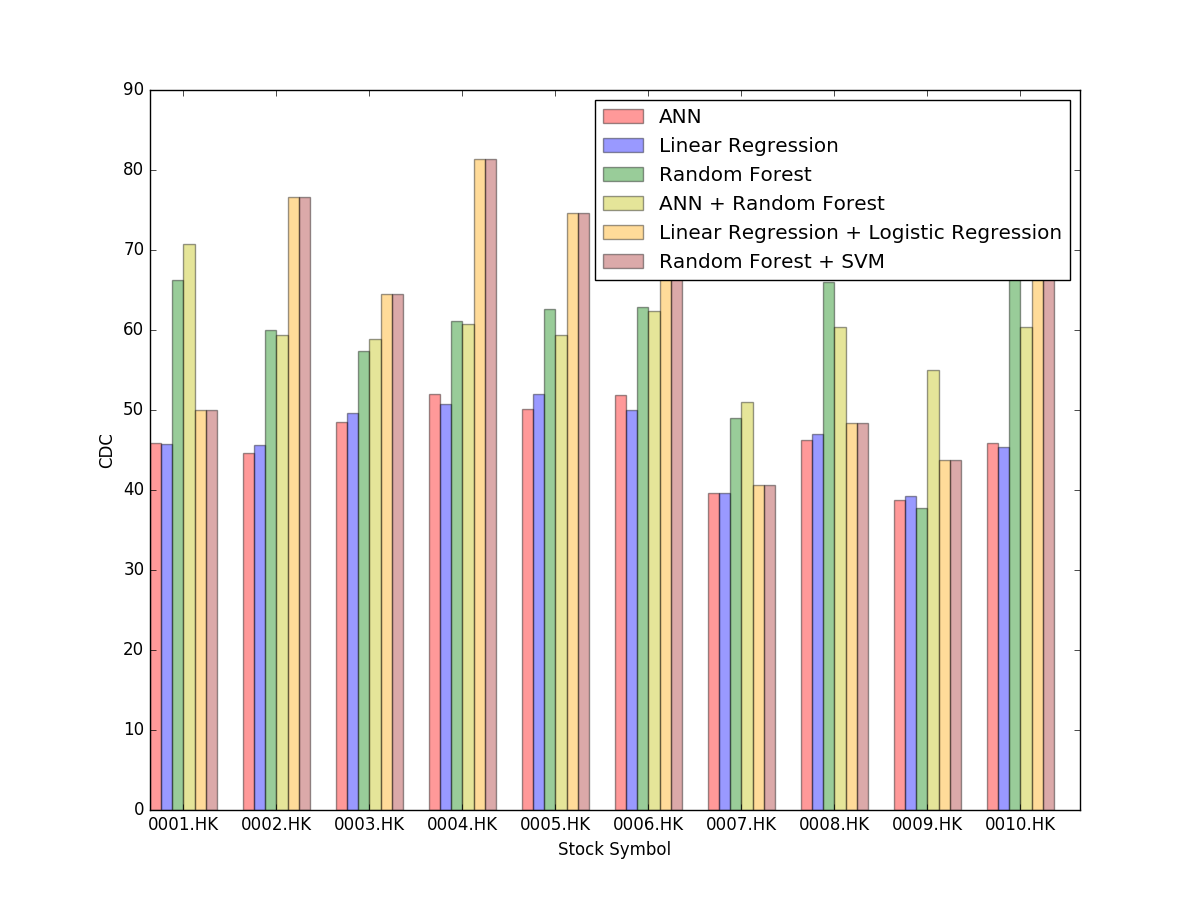
\includegraphics[width=.8\linewidth]{Result/3120102014/CDC}
	}
	\caption{Testing result in time period 2013-01-07 to 2014-01-06 (continue)}
	\label{fg:3yearpredict2}
\end{figure}

\begin{figure}[h]
	\centering
	\subfigure[MAPE]{
		\centering
		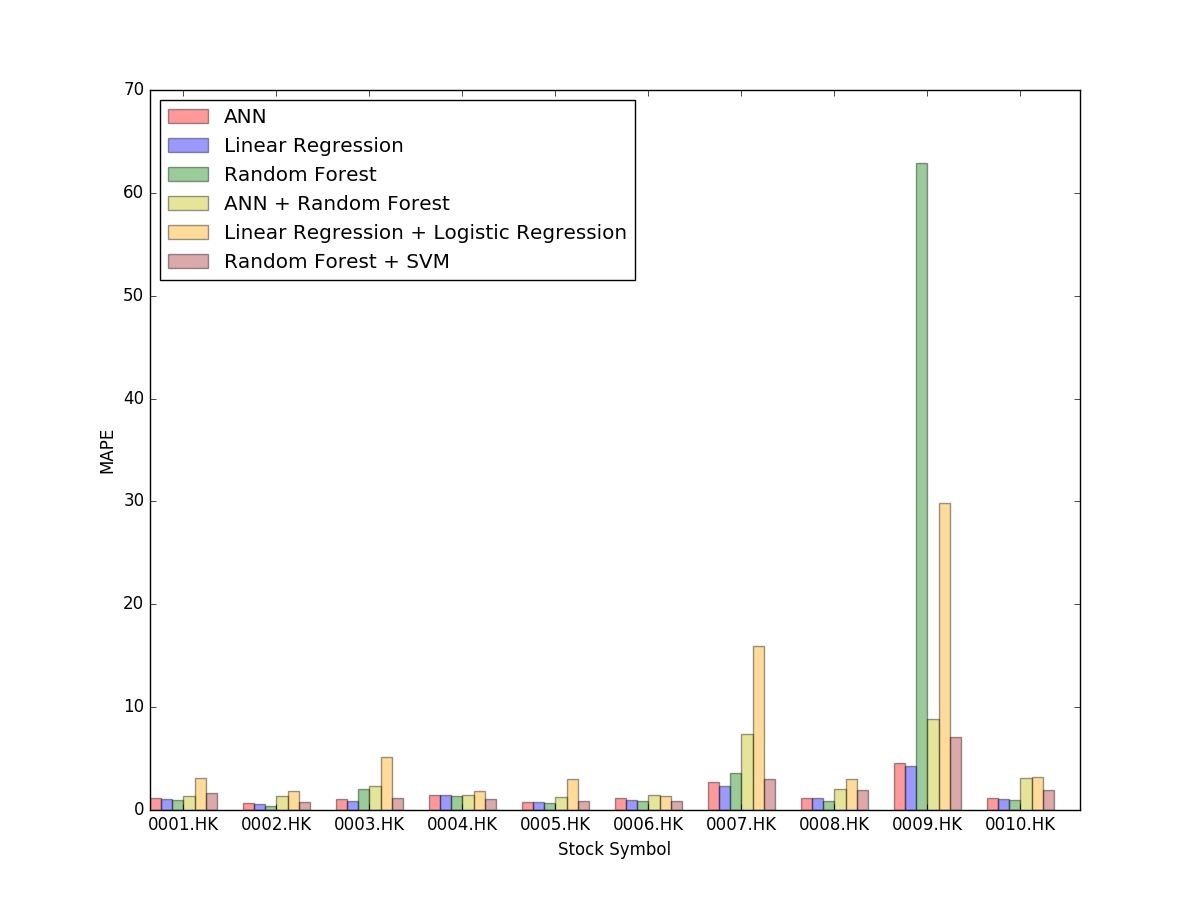
\includegraphics[width=.8\textwidth]{Result/3120102014/MAPE}
	}
	\subfigure[HMSE]{
		\centering
		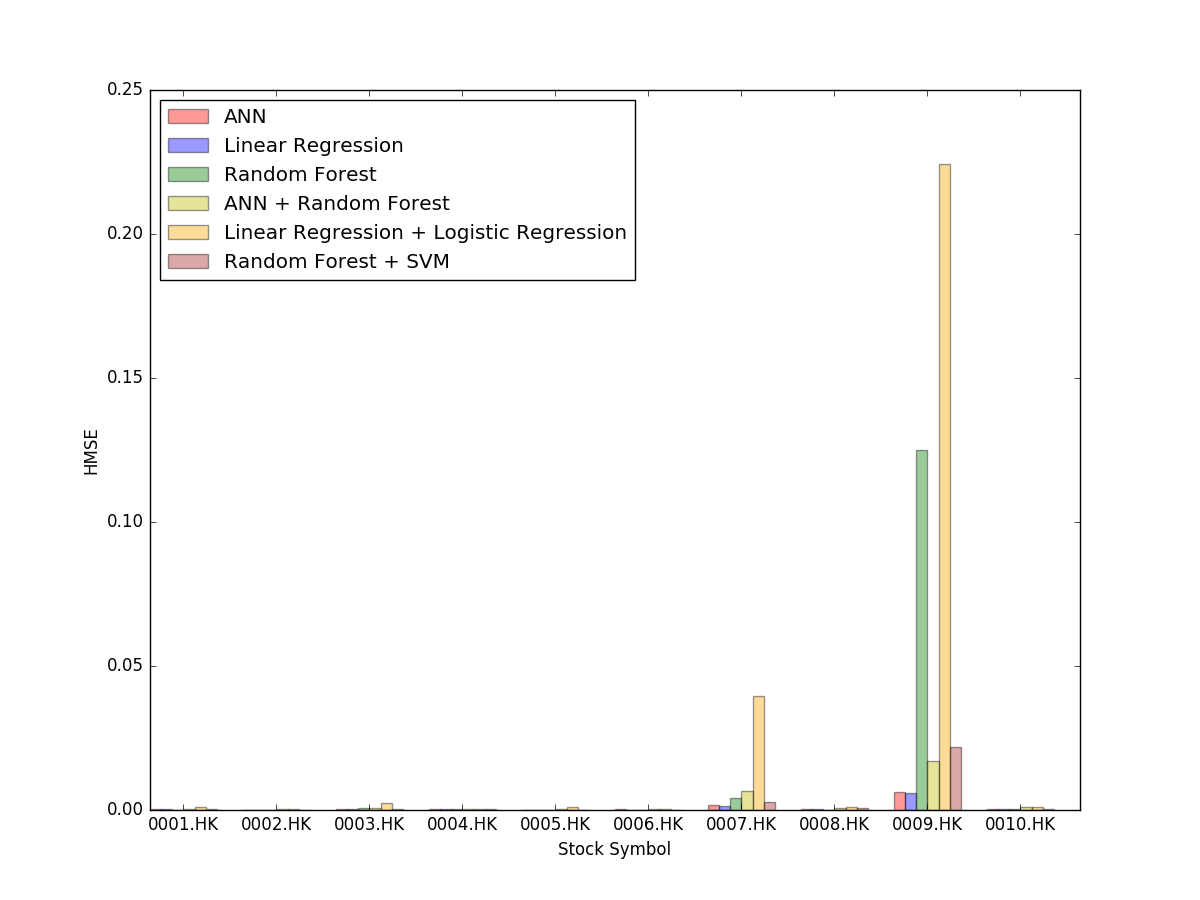
\includegraphics[width=.8\linewidth]{Result/3120102014/HMSE}
	}
	\caption{Testing result in time period 2013-01-07 to 2014-01-06 (continue)}
	\label{fg:3yearpredict3}
\end{figure}

\begin{table}[h]
	\centering
	\begin{tabular}{|l|l|}
		\hline
		\textbf{Algorithm} & \textbf{Average CDC} \\ \hline
		\textbf{ANN} & 46.33\% \\ \hline
		\textbf{Linear Regression} & 46.50\% \\ \hline
		\textbf{Random Forest} & 59.12\% \\ \hline
		\textbf{\begin{tabular}[c]{@{}l@{}}Linear Regression \\ + Logistic Regression\end{tabular}} & 63.55\% \\ \hline
		\textbf{Random Forest + SVM} & 63.54\% \\ \hline
		\textbf{ANN + Random Forest} & 65.82\% \\ \hline
	\end{tabular}
	\caption{Average CDC in time period 2013-01-07 to 2014-01-06}
	\label{tb:averageCDC2}
\end{table}
\clearpage

Composed learning model performed better in CDC test (in table~\ref{tb:averageCDC2}). Two linear classifiers share similar performance in this test. ANN and Linear Regression are also not trustworthy method to predict stock change direction\\

Random Forest alone and Linear + Logsitic Regression model turns out to be an unreliable choice to predict stock price in this test for some stock (like 0009.HK and 0007.HK). However, almost every method reach its worst performance when handle this two stocks, which on the other way shows that those model are not suitable for stock with average price less than.

\section{Using 2 years historical data}

The test slot is from 2010-01-06 to 2015-01-06, the first four year data (from 2012-01-06 to 2014-01-05) are training dataset (490 transaction days), the remaining used to act as testing data (test size is 248).\\

The average stock price over this period is showed in table~\ref{tb:avg20142015} and the RMSE comparison is in figure~\ref{fg:2yearpredict1} and \ref{fg:2yearpredict2}. Average CDC info can be found in table~\ref{tb:averageCDC3}.

\begin{table}[h]
	\centering
	\begin{tabular}{|l|l|}
		\hline
		\textbf{Algorithm} & \textbf{Average CDC} \\ \hline
		\textbf{ANN} & 46.12\% \\ \hline
		\textbf{Linear Regression} & 47.01\% \\ \hline
		\textbf{Random Forest} & 56.30\% \\ \hline
		\textbf{\begin{tabular}[c]{@{}l@{}}Linear Regression \\ + Logistic Regression\end{tabular}} & 62.22\% \\ \hline
		\textbf{Random Forest + SVM} & 62.18\% \\ \hline
		\textbf{ANN + Random Forest} & 58.12\% \\ \hline
	\end{tabular}
	\caption{Average CDC in time period 2014-01-06 to 2015-01-06}
	\label{tb:averageCDC3}
\end{table}

\begin{figure}[h]
	\centering
	\subfigure[ME]{
		\centering
		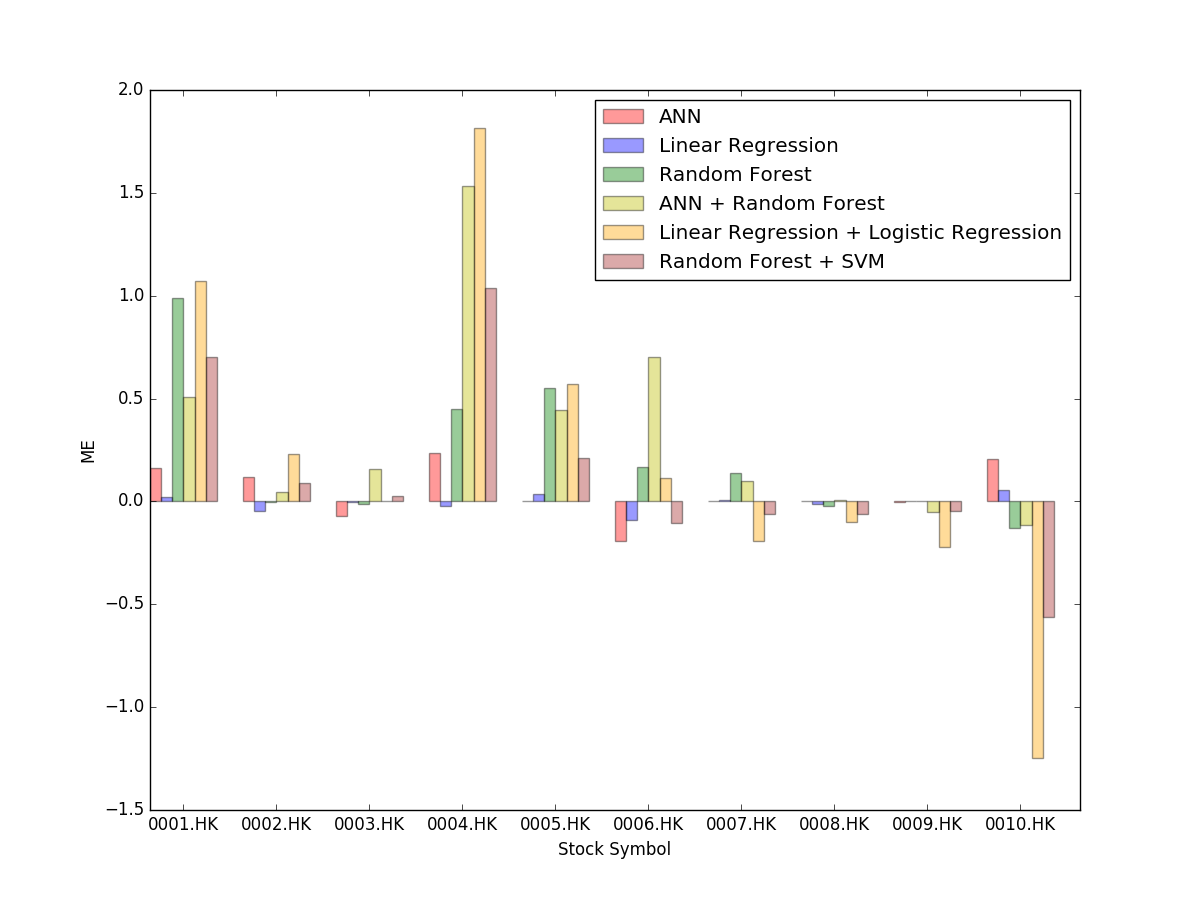
\includegraphics[width=.8\linewidth]{Result/20122015/ME}
	}
	\subfigure[MAPE]{
		\centering
		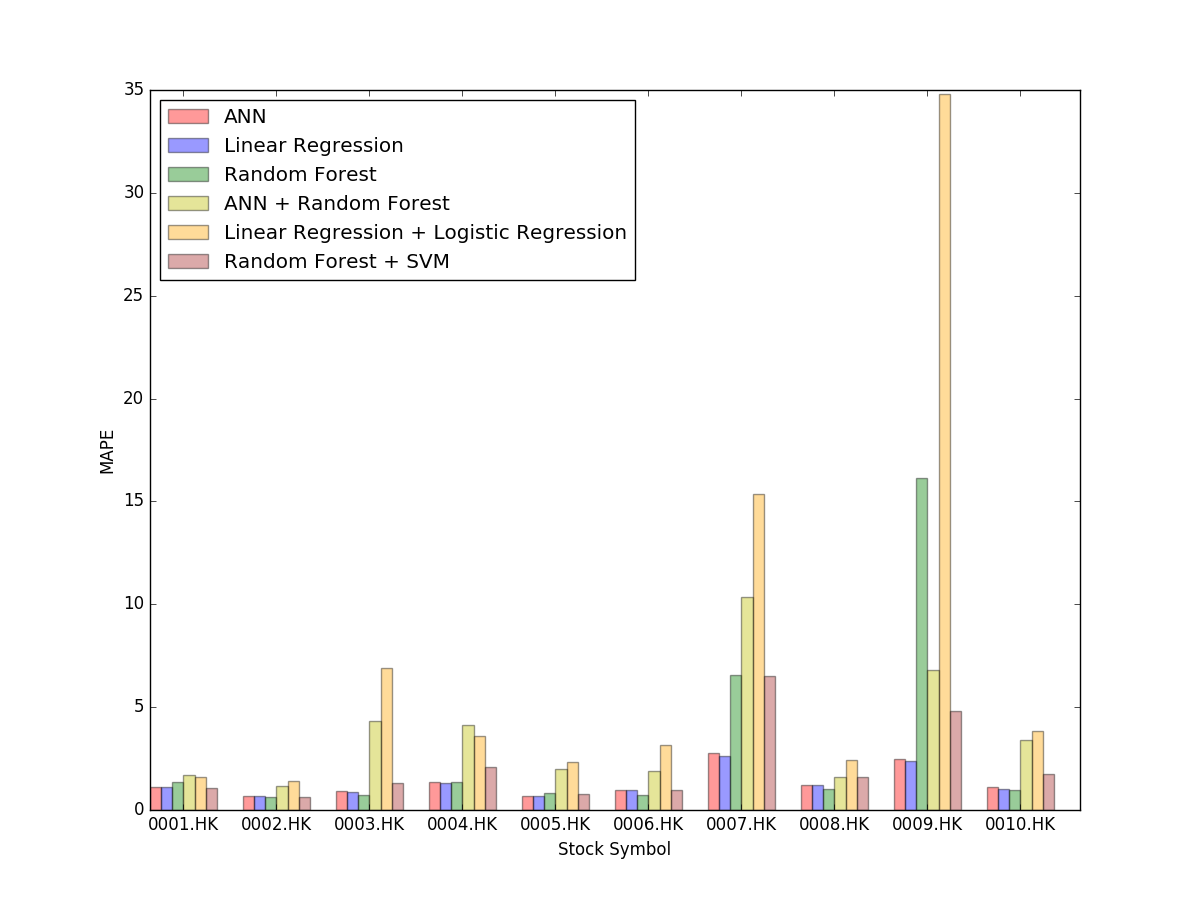
\includegraphics[width=.8\textwidth]{Result/20122015/MAPE}
	}
	\caption{Testing result in time period 2014-01-06 to 2015-01-06}
	\label{fg:2yearpredict1}
\end{figure}



\begin{figure}[h]
	\centering
	\subfigure[RMSE]{
		\centering
		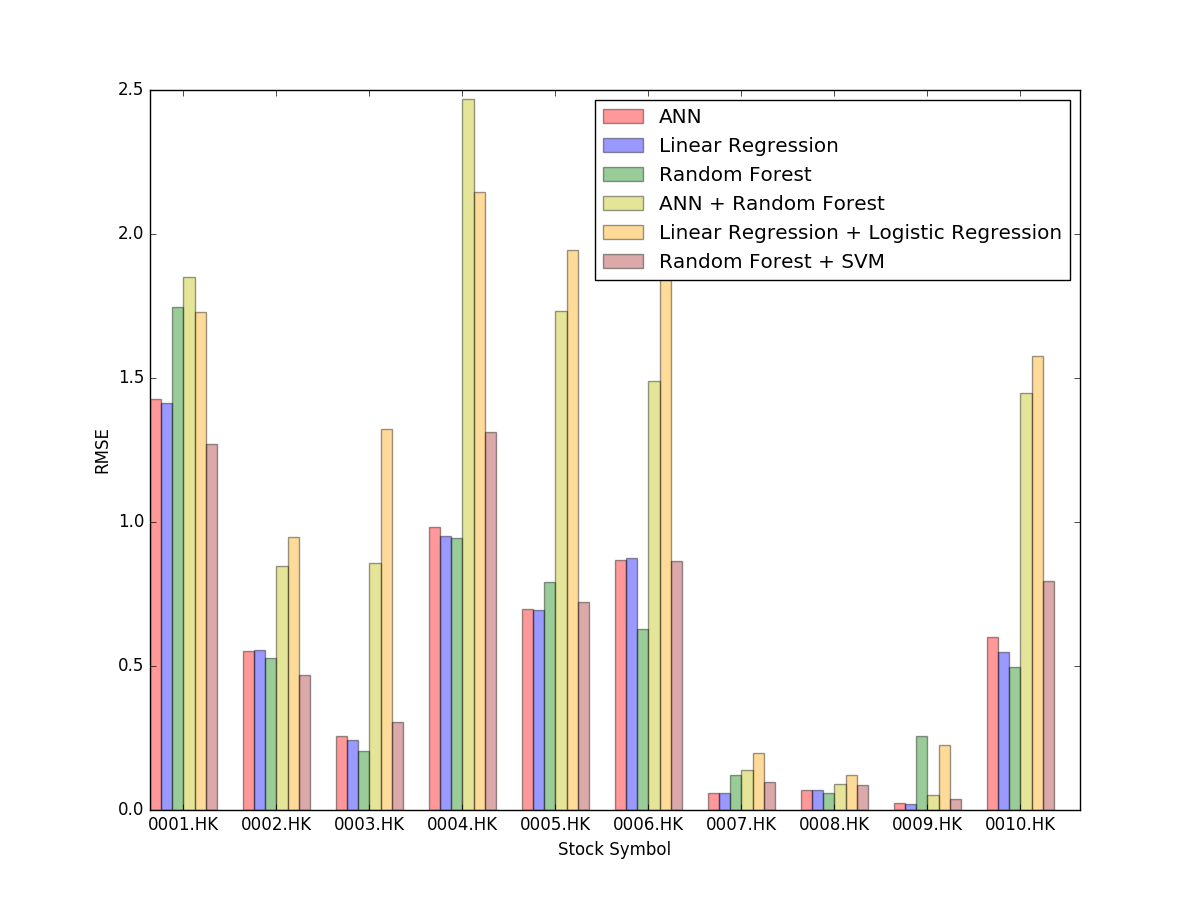
\includegraphics[width=.8\textwidth]{Result/20122015/RMSE}
	}
	\subfigure[CDC]{
		\centering
		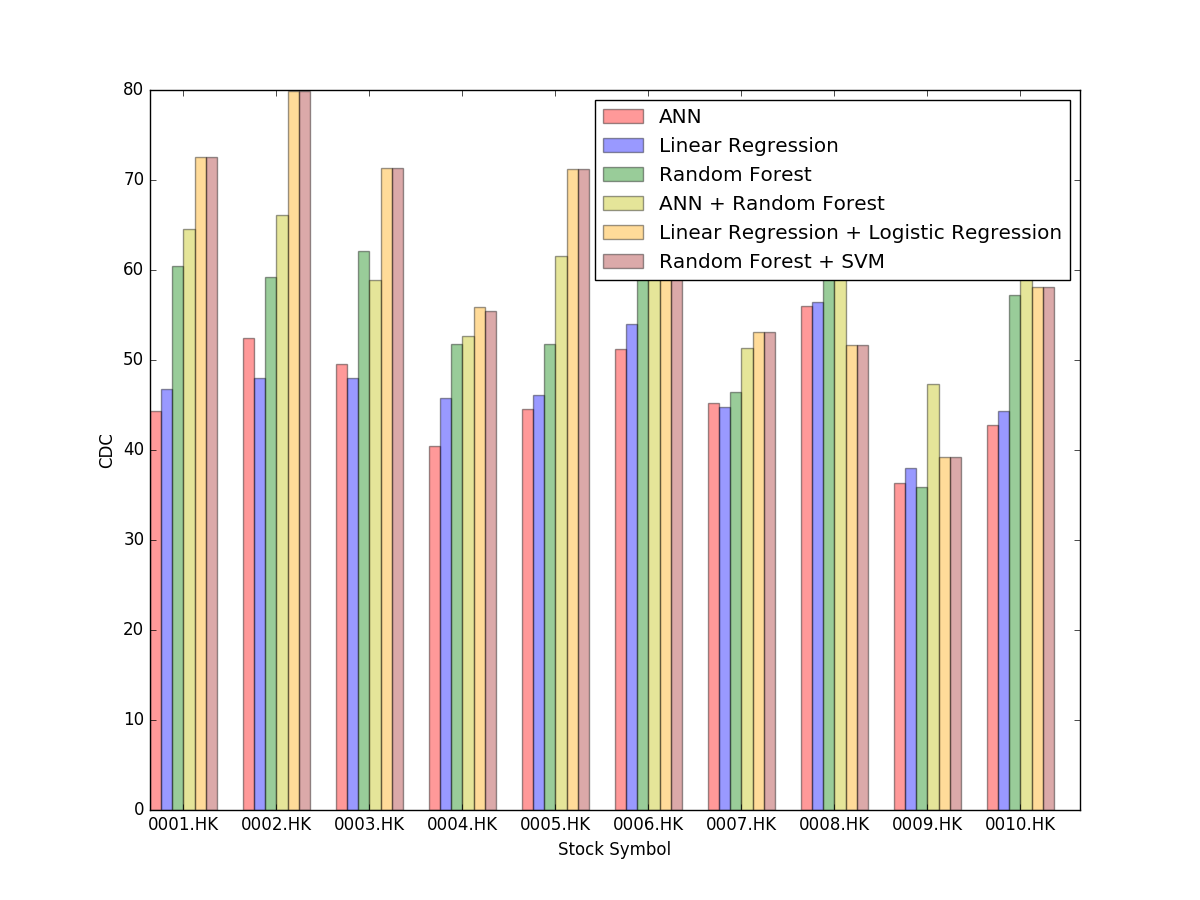
\includegraphics[width=.8\linewidth]{Result/20122015/CDC}
	}
	\caption{Testing result in time period 2014-01-06 to 2015-01-06 (continue)}
	\label{fg:2yearpredict2}
\end{figure}



\clearpage % Results and Discussion

\chapter{Conclusion}
\label{ch:conclusion}

This dissertation tested the predict performance of ANN, SVM, linear regression, logistic regression and random forest method with input different time period historical data to predict the behavior of all kinds of stocks in HKEX. The stock market is so complicated that it is difficult to precisely predict its behavior.\\


After the study, the best method in predicting stock price change amount is ANN, which performs well in performance test and shows great potential in distributed computing. The best method to predict stock change direction is Linear Regression and SVM (their performance are almost the same). Using two years historical data is enough to achieve the best performance. \\


In the future, there are still much improve space for distributed financial data forecaster,
\begin{itemize}
	\item \textbf{Explore the full potential of distributed computing power}. Limited to test environment, the running performance test does not complete. As using Numpy (non-distributed computing package) to compute matrix, ANN method also have some space to improve.
	\item \textbf{Mine the relationship between the input data and target stock more deeply}. One possible approach to do this is use specific data for different stock, e.g. using some raw materials price as input data while predict the stock behavior of manufacturers. Another method relies more on technical indicators.
	\item \textbf{Handle stock dividend and split}. This study just neglect this events. As there would be news beforehand, this type of error can be eliminated with proper design of system.
\end{itemize} % Conclusion

%% ----------------------------------------------------------------
% Now begin the Appendices, including them as separate files

\addtocontents{toc}{\vspace{2em}} % Add a gap in the Contents, for aesthetics

\appendix % Cue to tell LaTeX that the following 'chapters' are Appendices

\chapter{Technique Indicators}

\label{append:technical_indicator}

Technical analysis is one of the oldest security analysis methodology. A qualified technician predicts the direction of prices and makes buy or sell decision under the help of all kinds of charts and indicators.\\


This study also covers some indicators, the details of which can be find below.


\section{Moving Average (MA)\cite{kahn2006technical}}
A \textit{moving average} is the average price of a stock or market over a given period. MA helps neglect fluctuations and catch the main trend. Two basic type of MAs are used in this study.

\subsection{Simple Moving Average (SMA)}
SMA is the simplest MA. Assume that the price at time t is $ p_t $ where $t=1,2,3,\ldots$, $n$ is the given period, then the SMA at time $ t $ with $ n $ periods is
\begin{equation}
SMA(t, n)=\frac{\sum_{i=0}^{n-1}p_{t-i}}{n}
\end{equation}

\subsection{Exponential Moving Average (EMA)}  
SMA pays equal attention to every historical price. But, intuitively, the closer the stock price, the more significant it is in forecasting future price. To solve this problem, people developed EMA, which gives later prices higher weights than prior ones. Let $ K =\frac{2}{n+1} $, then EMA is 
\begin{equation}
EMA(t) = K\times p_t+(1-K) \times EMA(t-1)
\end{equation}

A comparison between EMA and SMA can be find in figure~\ref{fg:smaema}.
\begin{figure}[h]
	\centering
	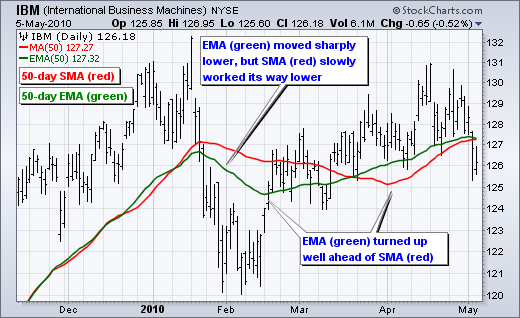
\includegraphics[width=0.8\textwidth]{EmaSma}
	\caption{Comparison between EMA and SMA\cite{9_sma_ema}}
	\label{fg:smaema}
\end{figure}

\section{Rate of Change (ROC)}
ROC is a simple way of measure the speed at which the price changes\cite{pring2002technical}. ROC can be calculated by
\begin{equation}
	ROC(n) = 100\times\frac{p_t}{p_{t-n}}
\end{equation}


\section{Relative Strength Index (RSI)}
RSI which was developed by Wells Wilder, measures change and speed of stock price relative strength\cite{pring2002technical}. The formula for RSI is
\begin{equation}
RSI = 100 - \frac{100}{1 + RS}
\end{equation}
where RS is
\begin{gather*}
RS=\frac{\text{Average Gain}}{\text{Average Loss}}\\
\end{gather*}
RSI value fluctuates in a constant range between 0 and 100. Usually, overbought and oversold lines are drawn at the 70 and 30 level\cite{pring2002technical}

\section{Moving Average Convergence Divergence (MACD)}
MACD measures the distance between two EMA lines (with different periods), and was developed by Gerald Appel\cite{kahn2006technical}. MACD can be calculted through,
\begin{equation}
MACD(m,n)=EMA(m)-EMA(n)
\end{equation}
Usually $ m < n $. The most widely used parameter for MACD is using 12-day EMA minus 26-day EMA\cite{kahn2006technical}.	% Introduction to Technical Indicators used in this thesis

\chapter{Introduction of company related in this dissertation}
\label{ch:stock_info}

Summary are collected from Yahoo Finance (http://finance.yahoo.com/), other information are from HKEX website (https://www.hkex.com.hk)


\section{CK Hutchison Holdings Ltd.}
\textbf{Symbol in Yahoo Finance}: 0001.HK\\
\textbf{Principal Activities}: Property development and investment, hotel and serviced suite operation, property and project management, and investment in infrastructure businesses and securities, ownership and leasing of movable assets.\\
\textbf{Industry Classification}: Conglomerates - Conglomerates - Conglomerates (HSIC*)
\paragraph{Summary}
Cheung Kong (Holdings) Limited, an investment holding company, is engaged in real estate property investment and development activities primarily in Hong Kong.


\section{CLP Holdings Ltd.}
\textbf{Symbol in Yahoo Finance}: 0002.HK\\
\textbf{Principal Activities}: Generation and supply of electricity in Hong Kong, India and Australia, and investment holding of power projects in Mainland China, Southeast Asia and Taiwan.\\
\textbf{Industry Classification}: Utilities - Utilities - Electricity (HSIC*)
\paragraph{Summary}
CLP Holdings Limited, an investment holding company, invests in, generates, and supplies electricity in Hong Kong, India, Australia, Mainland China, Southeast Asia, and Taiwan.


\section{Hong Kong and China Gas Co. Ltd., The}
\textbf{Symbol in Yahoo Finance}: 0003.HK\\
\textbf{Principal Activities}: Production, distribution and marketing of gas, water supply and emerging environmentally-friendly energy businesses in Hong Kong and the PRC; property development and investment activities in Hong Kong.\\
\textbf{Industry Classification}: Utilities - Utilities - Gas Distribution (HSIC*)
\paragraph{Summary}
The Hong Kong and China Gas Company Limited, together with its subsidiaries, engages in the production, distribution, and marketing of gas in Hong Kong and Mainland China.


\section{Wharf (Holdings) Ltd., The}
\textbf{Symbol in Yahoo Finance}: 0004.HK\\
\textbf{Principal Activities}: Investment property, development property, hotels operations, logistics and communications, media and entertainment.\\
\textbf{Industry Classification}: Properties \& Construction - Properties - Property Investment (HSIC*)
\paragraph{Summary}
The Wharf (Holdings) Limited, through its subsidiaries, engages in property and infrastructure investment in Hong Kong, Singapore, and the People's Republic of China.


\section{HSBC Holdings plc}
\textbf{Symbol in Yahoo Finance}: 0005.HK\\
\textbf{Principal Activities}: Provision of a comprehensive range of banking and related financial services through an int'l network in the Asia-Pacific region, Europe, the Americas, the Middle East and Africa.\\
\textbf{Industry Classification}: Financials - Banks - Banks (HSIC*)
\paragraph{Summary}
HSBC Holdings plc provides banking and financial products and services in the United Kingdom and internationally. It operates through Retail Banking and Wealth Management, Commercial Banking, Global Banking and Markets, and Global Private Banking .


\section{Power Assets Holdings Ltd.}
\textbf{Symbol in Yahoo Finance}: 0006.HK\\
\textbf{Principal Activities}: Generation and supply of electricity.\\
\textbf{Industry Classification}: Utilities - Utilities - Electricity (HSIC*)
\paragraph{Summary}
Power Assets Holdings Limited, an investment holding company, engages in the generation, transmission, and distribution of electricity in Hong Kong, the United Kingdom, Australia, Mainland China, and internationally.


\section{PCCW Ltd.}
\textbf{Symbol in Yahoo Finance}: 0008.HK\\
\textbf{Principal Activities}: Provision of telecommunication services, Internet and multimedia services, sale and rental of equipment and technical services. Investment in and development of infrastructure, properties and technology-related business.\\
\textbf{Industry Classification}: Telecommunications - Telecommunications - Telecommunication Services (HSIC*)
\paragraph{Summary}
PCCW Limited provides telecommunications services in Hong Kong, Mainland China, and internationally. The company's services include local telephony, local data and broadband, mobile and international telecommunications, and satellite-based an.


\section{Nine Express Ltd.}
\textbf{Symbol in Yahoo Finance}: 0009.HK\\
\textbf{Principal Activities}: Film distribution and licensing; film processing; rental of property; and property and hotel development.\\
\textbf{Industry Classification}: Properties \& Construction - Properties - Property Investment (HSIC*)


\section{Hang Lung Group Ltd.}
\textbf{Symbol in Yahoo Finance}: 0010.HK\\
\textbf{Principal Activities}: Property development for sale and leasing, property investment for rental income, operation of car park, property management and dry-cleaning.\\
\textbf{Industry Classification}: Properties \& Construction - Properties - Property Investment (HSIC*)
\paragraph{Summary}
Hang Lung Group Limited, an investment holding company, operates as property developer in Hong Kong and Mainland China. The company operates through Property Leasing and Property Sales segments.


\section{Hang Seng Bank Ltd.}
\textbf{Symbol in Yahoo Finance}: 0011.HK\\
\textbf{Principal Activities}: Provision of banking and related financial services.\\
\textbf{Industry Classification}: Financials - Banks - Banks (HSIC*)
\paragraph{Summary}
Hang Seng Bank Limited, together with its subsidiaries, provides banking and related financial services to individual, corporate, commercial, SME, and institutional customers in Hong Kong, rest of Asia-Pacific, and other countries.


\section{Henderson Land Development Co. Ltd.}
\textbf{Symbol in Yahoo Finance}: 0012.HK\\
\textbf{Principal Activities}: Property development and investment, construction, infrastructure, hotel operation, finance, department store operation, project management, investment holding and property management.\\
\textbf{Industry Classification}: Properties \& Construction - Properties - Property Development (HSIC*)
\paragraph{Summary}
Henderson Land Development Company Limited, an investment holding company, engages in the property development and investment activities in the People's Republic of China.


\section{None}
\textbf{Symbol in Yahoo Finance}: 0013.HK\\
\textbf{Principal Activities}: None\\
\textbf{Industry Classification}: None
\paragraph{Summary}
Hutchison Whampoa Limited, an investment holding company, operates in ports and related services, property and hotels, retail, infrastructure, energy, and mobile telecommunications businesses worldwide.


\section{Hysan Development Co. Ltd.}
\textbf{Symbol in Yahoo Finance}: 0014.HK\\
\textbf{Principal Activities}: Property investment, management and development.\\
\textbf{Industry Classification}: Properties \& Construction - Properties - Property Investment (HSIC*)
\paragraph{Summary}
Hysan Development Company Limited, together with its subsidiaries, engages in the investment, development, and management of properties in Hong Kong. It leases office, retail, and residential properties.


\section{Vantage International (Holdings) Ltd.}
\textbf{Symbol in Yahoo Finance}: 0015.HK\\
\textbf{Principal Activities}: Provision of construction, civil engineering, maintenance and other contract works in public and private sectors in Hong Kong, property investment and development.\\
\textbf{Industry Classification}: Properties \& Construction - Construction - Building Construction (HSIC*)
\paragraph{Summary}
Vantage International (Holdings) Limited, an investment holding company, engages in the construction, civil engineering, maintenance, and other contract works in public and private sectors in Hong Kong.


\section{Sun Hung Kai Properties Ltd.}
\textbf{Symbol in Yahoo Finance}: 0016.HK\\
\textbf{Principal Activities}: Development of and investment in properties for sale and rent, hotel operation, telecommunications, transportation, infrastructure and logistics.\\
\textbf{Industry Classification}: Properties \& Construction - Properties - Property Investment (HSIC*)
\paragraph{Summary}
Sun Hung Kai Properties Limited develops, sells, and rents real estate properties in Hong Kong, Mainland China, and internationally. The company's properties include residential projects, offices, industrial buildings, and shopping centers.


\section{New World Development Co. Ltd.}
\textbf{Symbol in Yahoo Finance}: 0017.HK\\
\textbf{Principal Activities}: Property investment and development, contracting, provision of services, infrastructure operations, telecommunication services, department store, hotel and restaurant operations and telecommunications, media and technology businesses.\\
\textbf{Industry Classification}: Properties \& Construction - Properties - Property Development (HSIC*)
\paragraph{Summary}
New World Development Company Limited, an investment holding company, invests in, develops, and manages properties in Hong Kong, Mainland China, and internationally.


\section{Oriental Press Group Ltd.}
\textbf{Symbol in Yahoo Finance}: 0018.HK\\
\textbf{Principal Activities}: Publication of newspapers.\\
\textbf{Industry Classification}: Consumer Services - Media \& Entertainment - Publishing (HSIC*)
\paragraph{Summary}
Oriental Press Group Limited, an investment holding company, engages in the publication of newspapers in Hong Kong and Australia. The company's flagship publication includes Oriental Daily News, a daily newspaper covering local and world news.


\section{Swire Pacific Ltd. 'A'}
\textbf{Symbol in Yahoo Finance}: 0019.HK\\
\textbf{Principal Activities}: Property, aviation, beverages, marine services and trading \& industrial.\\
\textbf{Industry Classification}: Conglomerates - Conglomerates - Conglomerates (HSIC*)
\paragraph{Summary}
Swire Pacific Limited engages in property, aviation, beverages, marine services, and trading and industrial businesses worldwide. Its Property Division develops, owns, and operates mixed-use properties.


\section{Wheelock and Co. Ltd.}
\textbf{Symbol in Yahoo Finance}: 0020.HK\\
\textbf{Principal Activities}: Investment property, development property, hotels, logistics and communications, media and entertainment.\\
\textbf{Industry Classification}: Properties \& Construction - Properties - Property Development (HSIC*)
\paragraph{Summary}
Wheelock and Company Limited, through its subsidiaries, engages in property investment, property development, and property management in Hong Kong and Singapore.


\section{Bank of East Asia, Ltd., The}
\textbf{Symbol in Yahoo Finance}: 0023.HK\\
\textbf{Principal Activities}: Provision of banking and related financial services, and business, corporate and investor services.\\
\textbf{Industry Classification}: Financials - Banks - Banks (HSIC*)
\paragraph{Summary}
The Bank of East Asia, Limited provides various banking and related financial services. It operates through nine segments: Personal Banking, Corporate Banking, Treasury Markets, Wealth Management, Financial Institutions, Others, China Operations, .


\section{Burwill Holdings Ltd.}
\textbf{Symbol in Yahoo Finance}: 0024.HK\\
\textbf{Principal Activities}: Trading of steel, processing of steel, mineral resources and commercial property.\\
\textbf{Industry Classification}: Materials - Diversified Metals \& Minerals - Iron \& Steel (HSIC*)
\paragraph{Summary}
Burwill Holdings Limited, an investment holding company, engages in the steel trading and processing businesses. Its International Steel Trading business is involved in the trading of iron ore fines and pellets, nickel ores, chrome ores, manganese.


\section{Chevalier International Holdings Ltd.}
\textbf{Symbol in Yahoo Finance}: 0025.HK\\
\textbf{Principal Activities}: Construction and engineering, insurance and investment, property, food and beverage. computer and information communication technology and others.\\
\textbf{Industry Classification}: Properties \& Construction - Construction - Building Construction (HSIC*)
\paragraph{Summary}
Chevalier International Holdings Limited, an investment holding company, engages in construction and engineering, insurance and investment, property, and food and beverage businesses.


\section{Galaxy Entertainment Group Ltd.}
\textbf{Symbol in Yahoo Finance}: 0027.HK\\
\textbf{Principal Activities}: Operation in casino games of chance or games of other forms, provision of hospitality and related services, and the manufacture, sale and distribution of construction materials.\\
\textbf{Industry Classification}: Consumer Services - Hotels, Casinos, Restaurants \& Leisure Facilities - Casinos \& Gaming (HSIC*)
\paragraph{Summary}
Galaxy Entertainment Group Limited, an investment holding company, develops and operates hotels, gaming, and integrated entertainment facilities in the Macau.


\section{China Aerospace International Holdings Ltd.}
\textbf{Symbol in Yahoo Finance}: 0031.HK\\
\textbf{Principal Activities}: Manufacturing and distribution of plastic products, liquid crystal display, printed circuit boards, intelligent chargers, polyimide films and other products; property investment and trading of electronic products.\\
\textbf{Industry Classification}: Industrials - Industrial Engineering - Industrial Components \& Equipment (HSIC*)
\paragraph{Summary}
China Aerospace International Holdings Limited, an investment holding company, manufactures and distributes technology products in the People's Republic of China and Canada.


\section{Cross-Harbour (Holdings) Ltd., The}
\textbf{Symbol in Yahoo Finance}: 0032.HK\\
\textbf{Principal Activities}: Operation of motoring schools, tunnels and an electronic toll collection system, and investment.\\
\textbf{Industry Classification}: Industrials - Industrial Transportation - Railway \& Tollroad Operation (HSIC*)
\paragraph{Summary}
The Cross-Harbour (Holdings) Limited, an investment holding company, operates motoring schools, tunnels, and an electronic toll collection system in Hong Kong.


\section{Kowloon Development Co. Ltd.}
\textbf{Symbol in Yahoo Finance}: 0034.HK\\
\textbf{Principal Activities}: Development and investment of property; and the holding of investments.\\
\textbf{Industry Classification}: Properties \& Construction - Properties - Property Development (HSIC*)
\paragraph{Summary}
Kowloon Development Company Limited, an investment holding company, engages in the investment, development, and management of properties. It operates through Property Development, Property Investment, Oil, and Others segments.


\section{Far East Consortium International Ltd.}
\textbf{Symbol in Yahoo Finance}: 0035.HK\\
\textbf{Principal Activities}: Property development, property investment, hotel operations and management, car park operations and securities and financial product investments.\\
\textbf{Industry Classification}: Properties \& Construction - Properties - Property Development (HSIC*)
\paragraph{Summary}
Far East Consortium International Limited, an investment holding company, engages in property development and investment, hospitality, and car park operations.


\section{First Tractor Co Ltd. - H Shares}
\textbf{Symbol in Yahoo Finance}: 0038.HK\\
\textbf{Principal Activities}: Manufacturing and selling agricultural machineries, diesel engines and fuel injections, other machineries and operating business of finance company.\\
\textbf{Industry Classification}: Industrials - Industrial Engineering - Heavy Industrial Machinery (HSIC*)
\paragraph{Summary}
First Tractor Company Limited engages in the research and development, manufacture, and sale of products agricultural machinery and powered machinery in the People's Republic of China and internationally.


\section{China Beidahuang Industry Group Holdings Ltd.}
\textbf{Symbol in Yahoo Finance}: 0039.HK\\
\textbf{Principal Activities}: Sales and distribution of wine and liquor; and production and sale of forages.\\
\textbf{Industry Classification}: Consumer Goods - Food \& Beverages - Alcohols (HSIC*)
\paragraph{Summary}
China Beidahuang Industry Group Holdings Limited, an investment holding company, engages in the wine and liquor, green food products sales, animal feed, logistic warehouse, and money lending businesses in the People's Republic of China.


\section{Great Eagle Holdings Ltd.}
\textbf{Symbol in Yahoo Finance}: 0041.HK\\
\textbf{Principal Activities}: Property development and investment, hotel and restaurant operations, manager of REIT, trading of building materials, share investment, provision of management and maintenance services, property management and fitness centre operation.\\
\textbf{Industry Classification}: Properties \& Construction - Properties - Property Investment (HSIC*)
\paragraph{Summary}
Great Eagle Holdings Limited, an investment holding company, develops, invests in, and manages residential, office, retail, and hotel properties in Asia, North America, Australasia, and Europe.


\section{Northeast Electric Development Co. Ltd. - H Shares}
\textbf{Symbol in Yahoo Finance}: 0042.HK\\
\textbf{Principal Activities}: Production and sales of power transmission equipment and related accessories, provision of relevant after-sale services, and provision of power transmission technology developing, consulting, transferring and testing services.\\
\textbf{Industry Classification}: Industrials - Industrial Engineering - Industrial Components \& Equipment (HSIC*)
\paragraph{Summary}
Northeast Electric Development Company Limited produces and sells power transmission equipment and related accessories. The company primarily offers switchgears, power capacitors, enclosed bus bars, and other system protection and transmission equ.


\section{C. P. Pokphand Co. Ltd.}
\textbf{Symbol in Yahoo Finance}: 0043.HK\\
\textbf{Principal Activities}: Manufacture and sale of animal feed products; breeding, farming and sale of livestock, aquatic animals and value-added processed food products.\\
\textbf{Industry Classification}: Consumer Goods - Agricultural Products - Animal Feeds (HSIC*)
\paragraph{Summary}
C.P. Pokphand Co. Ltd., an investment holding company, manufactures and sells animal feed products in the People's Republic of China and the Socialist Republic of Vietnam.


\section{Hong Kong Aircraft Engineering Co. Ltd.}
\textbf{Symbol in Yahoo Finance}: 0044.HK\\
\textbf{Principal Activities}: Commercial aircraft overhaul, modification and maintenance.\\
\textbf{Industry Classification}: Consumer Services - Transportation - Airlines (HSIC*)
\paragraph{Summary}
Hong Kong Aircraft Engineering Company Limited provides commercial aircraft overhaul, modification, and maintenance services to airlines in Hong Kong, Mainland China, and the United States.


\section{Hongkong and Shanghai Hotels, Ltd., The}
\textbf{Symbol in Yahoo Finance}: 0045.HK\\
\textbf{Principal Activities}: Ownership, development, and management of prestigious hotels and commercial and residential properties in Asia, the United States and Europe; and provision of tourism and leisure, club management and other services.\\
\textbf{Industry Classification}: Consumer Services - Hotels, Casinos, Restaurants \& Leisure Facilities - Hotels \& Resorts (HSIC*)
\paragraph{Summary}
The Hongkong and Shanghai Hotels, Limited, an investment holding company, owns, develops, and manages hotels, and commercial and residential properties in Asia, the United States, and Europe.


\section{Fairwood Holdings Ltd.}
\textbf{Symbol in Yahoo Finance}: 0052.HK\\
\textbf{Principal Activities}: Operation of fast food restaurants and property investments.\\
\textbf{Industry Classification}: Consumer Services - Hotels, Casinos, Restaurants \& Leisure Facilities - Restaurants (HSIC*)
\paragraph{Summary}
Fairwood Holdings Limited, an investment holding company, engages in the operation of fast food restaurants. The company operates through two segments, Hong Kong Restaurants and Mainland China Restaurants.


\section{Guoco Group Ltd.}
\textbf{Symbol in Yahoo Finance}: 0053.HK\\
\textbf{Principal Activities}: Proprietary asset management, property development and investment, hospitality and leisure business, stock and commodity broking, investment advisory, banking and financing, insurance, fund management and merchant banking.\\
\textbf{Industry Classification}: Financials - Other Financials - Investment \& Asset Management (HSIC*)
\paragraph{Summary}
Guoco Group Limited, an investment holding company, engages in property development and investment, hospitality and leisure, stock and commodity broking, and investment advisory businesses.


\section{Hopewell Holdings Ltd.}
\textbf{Symbol in Yahoo Finance}: 0054.HK\\
\textbf{Principal Activities}: Investment in toll roads and power plant, property development and investment, property agency and management, hotel ownership and management, restaurant operations and food catering.\\
\textbf{Industry Classification}: Conglomerates - Conglomerates - Conglomerates (HSIC*)
\paragraph{Summary}
Hopewell Holdings Limited, an investment holding company, engages in the investment in infrastructure projects, property development and investment, property agency and management, hotel investment and management, restaurant operations, and food c.


\section{Allied Properties (HK) Ltd.}
\textbf{Symbol in Yahoo Finance}: 0056.HK\\
\textbf{Principal Activities}: Investment, broking and finance, consumer finance, property rental, hotel operations and management services, sales of properties and property based investments.\\
\textbf{Industry Classification}: Financials - Other Financials - Financing (HSIC*)
\paragraph{Summary}
Allied Properties (H.K.) Limited, an investment holding company, engages in property investment, property development, financial services, and hospitality related activities in Hong Kong, Mainland China, and internationally.


\section{Chen Hsong Holdings Ltd.}
\textbf{Symbol in Yahoo Finance}: 0057.HK\\
\textbf{Principal Activities}: Manufacture and sale of plastic injection moulding machines and related products.\\
\textbf{Industry Classification}: Industrials - Industrial Engineering - Industrial Components \& Equipment (HSIC*)
\paragraph{Summary}
Chen Hsong Holdings Limited manufactures and sells plastic injection molding machines and related products in Mainland China, Hong Kong, Taiwan, and internationally.


\section{Transport International Holdings Ltd.}
\textbf{Symbol in Yahoo Finance}: 0062.HK\\
\textbf{Principal Activities}: Operation of both franchised and non-franchised public transportation, property holdings and development and the provision of media sales services.\\
\textbf{Industry Classification}: Consumer Services - Transportation - Public Transport (HSIC*)
\paragraph{Summary}
Transport International Holdings Limited, an investment holding company, provides franchised and non-franchised public transportation services in the People's Republic of China.


\section{Get Nice Holdings Ltd.}
\textbf{Symbol in Yahoo Finance}: 0064.HK\\
\textbf{Principal Activities}: Provision of securities dealing and broking, futures and options broking, underwriting and placements, securities margin financing, money lending, corporate finance services; property holding and investments in financial instruments.\\
\textbf{Industry Classification}: Financials - Other Financials - Securities \& Brokerage (HSIC*)
\paragraph{Summary}
Get Nice Holdings Limited, an investment holding company, provides various financial services in Hong Kong. It operates through five divisions: Broking, Securities Margin Financing, Money Lending, Corporate Finance, and Investments.


\section{Grand Ocean Advanced Resources Co. Ltd.}
\textbf{Symbol in Yahoo Finance}: 0065.HK\\
\textbf{Principal Activities}: Manufacturing and sale of plastic woven bags, paper bags and plastic barrels, sale of coal and provision of low-rank coal upgrading services.\\
\textbf{Industry Classification}: Energy - Coal - Coal (HSIC*)
\paragraph{Summary}
Grand Ocean Advanced Resources Company Limited, an investment holding company, manufactures and sells plastic woven bags, paper bags, and plastic barrels in Hong Kong and the People's Republic of China.


\section{MTR Corporation Ltd.}
\textbf{Symbol in Yahoo Finance}: 0066.HK\\
\textbf{Principal Activities}: Railway design, construction, operation, maintenance and investment in Hong Kong, the Mainland of China and overseas cities; project management; station commercial business; property business; and investment in Octopus Holdings Limited.\\
\textbf{Industry Classification}: Consumer Services - Transportation - Public Transport (HSIC*)
\paragraph{Summary}
MTR Corporation Limited designs, constructs, operates, maintains, and invests railways in Hong Kong, the Mainland China, and internationally. The company operates a rail-based transportation system in Hong Kong, comprising domestic and cross-bound.


\section{Tai Cheung Holdings Ltd.}
\textbf{Symbol in Yahoo Finance}: 0088.HK\\
\textbf{Principal Activities}: Property investment and development, investment holding and property management.\\
\textbf{Industry Classification}: Properties \& Construction - Properties - Property Development (HSIC*)
\paragraph{Summary}
Tai Cheung Holdings Limited, an investment holding company, engages in property investment, development, and management activities in Hong Kong. It develops various properties, including office, commercial, industrial/godown, residential, and car .


\section{Cosmopolitan International Holdings Ltd.}
\textbf{Symbol in Yahoo Finance}: 0120.HK\\
\textbf{Principal Activities}: Property development and investment, and financial assets and other investments.\\
\textbf{Industry Classification}: Properties \& Construction - Properties - Property Development (HSIC*)
\paragraph{Summary}
Cosmopolitan International Holdings Limited, an investment holding company, develops and invests in real estate properties in Hong Kong. It operates through two segments, Property Development and Investment, and Financial Assets Investments.


\section{Tsingtao Brewery Co. Ltd. - H Shares}
\textbf{Symbol in Yahoo Finance}: 0168.HK\\
\textbf{Principal Activities}: Production, sales and domestic trade of beer.\\
\textbf{Industry Classification}: Consumer Goods - Food \& Beverages - Alcohols (HSIC*)
\paragraph{Summary}
Tsingtao Brewery Company Limited, together with its subsidiaries, engages in the production, distribution, wholesale, and retail sale of beer products primarily in the People's Republic of China.


\section{Kingdee International Software Group Co. Ltd.}
\textbf{Symbol in Yahoo Finance}: 0268.HK\\
\textbf{Principal Activities}: Developing, manufacturing and selling of enterprise management software products and provision of software-related technical services in the PRC.\\
\textbf{Industry Classification}: Information Technology - Software \& Services - Software (HSIC*)
\paragraph{Summary}
Kingdee International Software Group Company Limited, an investment holding company, develops, manufactures, markets, and sells enterprise management software products.


\section{China Resources Beer (Holdings) Co. Ltd.}
\textbf{Symbol in Yahoo Finance}: 0291.HK\\
\textbf{Principal Activities}: Manufacturing, sales and distribution of beer products.\\
\textbf{Industry Classification}: Consumer Goods - Food \& Beverages - Alcohols (HSIC*)
\paragraph{Summary}
China Resources Beer (Holdings) Company Limited, an investment holding company, manufactures, sells, and distributes beer products in Hong Kong, Mainland China, and internationally.


\section{Tianda Pharmaceuticals Ltd.}
\textbf{Symbol in Yahoo Finance}: 0455.HK\\
\textbf{Principal Activities}: Research and development, production and sales of pharmaceutical, biotechnology and healthcare products.\\
\textbf{Industry Classification}: Consumer Goods - Healthcare - Pharmaceuticals (HSIC*)
\paragraph{Summary}
Tianda Pharmaceuticals Limited, an investment holding company, engages in the research and development, production, and sale of pharmaceutical, biotechnology, and healthcare products.


\section{CMMB Vision Holdings Ltd.}
\textbf{Symbol in Yahoo Finance}: 0471.HK\\
\textbf{Principal Activities}: Provision of China Mobile Multimedia Broadcasting services and trading of printed circuit board materials.\\
\textbf{Industry Classification}: Telecommunications - Telecommunications - Satellite \& Wireless Communication (HSIC*)
\paragraph{Summary}
CMMB Vision Holdings Limited, an investment holding company, engages in the transmission and broadcasting of television (TV) programs. It operates through CMMB Business and Trading Business segments.


\section{Fufeng Group Ltd.}
\textbf{Symbol in Yahoo Finance}: 0546.HK\\
\textbf{Principal Activities}: Manufacture and sales of fermentation-based food additive and biochemical products and starch-based products.\\
\textbf{Industry Classification}: Consumer Goods - Food \& Beverages - Food Additives (HSIC*)
\paragraph{Summary}
Fufeng Group Limited, an investment holding company, engages in the manufacture and sale of fermentation-based food additive and biochemical products, and starch-based products in the People's Republic of China.


\section{The 13 Holdings Ltd.}
\textbf{Symbol in Yahoo Finance}: 0577.HK\\
\textbf{Principal Activities}: Management contracting, property development management, property investment and hotel development.\\
\textbf{Industry Classification}: Properties \& Construction - Construction - Building Construction (HSIC*)
\paragraph{Summary}
The 13 Holdings Limited, an investment holding company, operates as a hospitality, entertainment, and construction group in the People's Republic of China and Singapore.


\section{China Overseas Land \& Investment Ltd.}
\textbf{Symbol in Yahoo Finance}: 0688.HK\\
\textbf{Principal Activities}: Property development and investment, real estate management and treasury operations.\\
\textbf{Industry Classification}: Properties \& Construction - Properties - Property Development (HSIC*)
\paragraph{Summary}
China Overseas Land \& Investment Limited, an investment holding company, engages in the property development and investment, real estate agency and management, and treasury operations.


\section{Tencent Holdings Ltd.}
\textbf{Symbol in Yahoo Finance}: 0700.HK\\
\textbf{Principal Activities}: Provision of Internet and mobile value-added services, online advertising services and eCommerce transactions services to users in the PRC.\\
\textbf{Industry Classification}: Information Technology - Software \& Services - E-Commerce \& Internet Services (HSIC*)
\paragraph{Summary}
Tencent Holdings Limited, an investment holding company, provides Internet and mobile value-added services (VAS), and online advertising services in Mainland China, the United States, Europe, and internationally.


\section{Hopewell Highway Infrastructure Ltd.}
\textbf{Symbol in Yahoo Finance}: 0737.HK\\
\textbf{Principal Activities}: Initiate, promote, develop and operate strategically important roads, tunnels, bridges and related infrastructure projects in the PRC.\\
\textbf{Industry Classification}: Industrials - Industrial Transportation - Railway \& Tollroad Operation (HSIC*)
\paragraph{Summary}
Hopewell Highway Infrastructure Limited, an investment holding company, develops and operates expressways in Guangdong Province, the People's Republic of China.


\section{China National Culture Group Ltd.}
\textbf{Symbol in Yahoo Finance}: 0745.HK\\
\textbf{Principal Activities}: Advertising and movie production.\\
\textbf{Industry Classification}: Consumer Services - Media \& Entertainment - Advertising \& Marketing (HSIC*)
\paragraph{Summary}
China National Culture Group Limited, an investment holding company, engages in the production and distribution of films in the People's Republic of China.


\section{NetDragon Websoft Holdings Ltd.}
\textbf{Symbol in Yahoo Finance}: 0777.HK\\
\textbf{Principal Activities}: Online games development, including games design, programming and graphics and online games operation; education business; and mobile solution and mobile marketing business.\\
\textbf{Industry Classification}: Information Technology - Software \& Services - Software (HSIC*)
\paragraph{Summary}
NetDragon Websoft Holdings Limited, an investment holding company, designs, develops, programs, and operates online games primarily in the People's Republic of China, the United States, and internationally.


\section{Glorious Property Holdings Ltd.}
\textbf{Symbol in Yahoo Finance}: 0845.HK\\
\textbf{Principal Activities}: Develop and sale of high quality properties in key economic cities in the PRC.\\
\textbf{Industry Classification}: Properties \& Construction - Properties - Property Development (HSIC*)
\paragraph{Summary}
Glorious Property Holdings Limited, an investment holding company, develops and sells large-scale real estate properties in the People's Republic of China.


\section{TUS International Ltd.}
\textbf{Symbol in Yahoo Finance}: 0872.HK\\
\textbf{Principal Activities}: Design, research and development, manufacture and sale of automotive electronic products and automotive safety spare parts, the premium car (including classic car) investment \& trading business \& investment business in property in the PRC.\\
\textbf{Industry Classification}: Consumer Goods - Automobiles - Auto Parts (HSIC*)
\paragraph{Summary}
TUS International Limited, an investment holding company, produces and sells automotive electronic products and safety spare parts in the People's Republic of China.


\section{RoadShow Holdings Ltd.}
\textbf{Symbol in Yahoo Finance}: 0888.HK\\
\textbf{Principal Activities}: Provision of media sales \& design services \& production of advertisements for Multimedia On-board, transit vehicle exteriors \& interiors, online portal, mobile apps, shelters \& outdoor signages advertising, integrated marketing services.\\
\textbf{Industry Classification}: Consumer Services - Media \& Entertainment - Broadcasting (HSIC*)
\paragraph{Summary}
RoadShow Holdings Limited, an investment holding company, engages in multi-media on-board (MMOB), transit network, and merchandising businesses in Hong Kong and Mainland China.


\section{G-Resources Group Ltd.}
\textbf{Symbol in Yahoo Finance}: 1051.HK\\
\textbf{Principal Activities}: Exploration and mining, sale of gold and silver products.\\
\textbf{Industry Classification}: Materials - Gold \& Precious Metals - Gold \& Precious Metals (HSIC*)
\paragraph{Summary}
G-Resources Group Limited, an investment holding company, explores and mines mineral properties, primarily gold. It operates through Principal Investment Business, Money Lending Business, Real Property Business, and Mining Business.


\section{Biostime International Holdings Ltd.}
\textbf{Symbol in Yahoo Finance}: 1112.HK\\
\textbf{Principal Activities}: Manufacture and sale of premium pediatric nutritional and baby care products and adult nutrition supplements and skincare products.\\
\textbf{Industry Classification}: Consumer Goods - Food \& Beverages - Packaged Foods (HSIC*)
\paragraph{Summary}
Biostime International Holdings Limited, an investment holding company, provides pediatric nutritional and baby care products to mothers primarily in the People's Republic of China.


\section{China Modern Dairy Holdings Ltd.}
\textbf{Symbol in Yahoo Finance}: 1117.HK\\
\textbf{Principal Activities}: Production and sale of raw milk to customers for processing into dairy products; and production and sale of liquid milk products.\\
\textbf{Industry Classification}: Consumer Goods - Food \& Beverages - Dairy Products (HSIC*)
\paragraph{Summary}
China Modern Dairy Holdings Ltd., an investment holding company, produces and sells raw milk and liquid milk products in the People's Republic of China.


\section{China-Hongkong Photo Products Holdings Ltd.}
\textbf{Symbol in Yahoo Finance}: 1123.HK\\
\textbf{Principal Activities}: Marketing and distribution of photographic developing, processing and printing products \& sale of photographic merchandises, skincare products, consumer electronic products and household appliances; and provision of technical services.\\
\textbf{Industry Classification}: Consumer Goods - Household Goods \& Electronics - Consumer Electronics (HSIC*)
\paragraph{Summary}
China-Hongkong Photo Products Holdings Limited, an investment holding company, engages in marketing and distributing photographic developing, processing, and printing products primarily in Hong Kong and the People's Republic of China.


\section{Tang Palace (China) Holdings Ltd.}
\textbf{Symbol in Yahoo Finance}: 1181.HK\\
\textbf{Principal Activities}: Restaurant operations and food productions.\\
\textbf{Industry Classification}: Consumer Services - Hotels, Casinos, Restaurants \& Leisure Facilities - Restaurants (HSIC*)
\paragraph{Summary}
Tang Palace (China) Holdings Limited, an investment holding company, engages in the restaurant and food production business in the People's Republic of China.


\section{Yashili International Holdings Ltd.}
\textbf{Symbol in Yahoo Finance}: 1230.HK\\
\textbf{Principal Activities}: Manufacture and sale of dairy and nourishment products.\\
\textbf{Industry Classification}: Consumer Goods - Food \& Beverages - Packaged Foods (HSIC*)
\paragraph{Summary}
Yashili International Holdings Ltd, an investment holding company, manufactures and sells dairy and nourishment products in the People's Republic of China and internationally.


\section{SPT Energy Group Inc.}
\textbf{Symbol in Yahoo Finance}: 1251.HK\\
\textbf{Principal Activities}: Provision of oilfield services including drilling, well completion, reservoir, with ancillary activities in trading and manufacturing of oil field services related products.\\
\textbf{Industry Classification}: Energy - Oil \& Gas - Oil \& Gas Equipment \& Services (HSIC*)
\paragraph{Summary}
SPT Energy Group Inc., an investment holding company, provides integrated oilfield services and related products in the People's Republic of China, the Republic of Kazakhstan, Singapore, and Canada.


\section{Tsui Wah Holdings Ltd.}
\textbf{Symbol in Yahoo Finance}: 1314.HK\\
\textbf{Principal Activities}: Provision of food catering services through a chain of Hong Kong-style restaurants in Hong Kong and the PRC.\\
\textbf{Industry Classification}: Consumer Services - Hotels, Casinos, Restaurants \& Leisure Facilities - Restaurants (HSIC*)
\paragraph{Summary}
Tsui Wah Holdings Limited, an investment holding company, operates a chain of Cha Chaan Teng restaurants. It provides food catering services through a chain of Hong Kong-style restaurants.


\section{361 Degrees International Ltd.}
\textbf{Symbol in Yahoo Finance}: 1361.HK\\
\textbf{Principal Activities}: Manufacturing and sales of sporting goods, including footwear, apparel and accessories in the PRC.\\
\textbf{Industry Classification}: Consumer Goods - Textiles, Clothing \& Personal Care - Footwear (HSIC*)
\paragraph{Summary}
361 Degrees International Limited, an investment holding company, manufactures and trades adults sporting goods primarily in the People's Republic of China.


\section{Synertone Communication Corporation}
\textbf{Symbol in Yahoo Finance}: 1613.HK\\
\textbf{Principal Activities}: Design, research \& development, manufacture \& sales of communication systems, equipment \& systems technologies; providing total solution of communication system; provision of satellite bandwidth capacity \& communication service application.\\
\textbf{Industry Classification}: Information Technology - IT Hardware - Telecommunication Equipment (HSIC*)
\paragraph{Summary}
Synertone Communication Corporation designs, researches and develops, manufactures, and sells specialized communication systems, equipment, and systems technologies in the People's Republic of China.


\section{Sunac China Holdings Ltd.}
\textbf{Symbol in Yahoo Finance}: 1918.HK\\
\textbf{Principal Activities}: Property development, property investment and property management services.\\
\textbf{Industry Classification}: Properties \& Construction - Properties - Property Development (HSIC*)
\paragraph{Summary}
Sunac China Holdings Limited, together with its subsidiaries, develops residential and commercial properties in the People's Republic of China. Its property portfolio includes high-rise and mid-rise apartments, detached villas, townhouses, re.


\section{SSY Group Ltd.}
\textbf{Symbol in Yahoo Finance}: 2005.HK\\
\textbf{Principal Activities}: Research, development, manufacturing and selling of a wide range of finished medicines, bulk pharmaceutical products and medical materials.\\
\textbf{Industry Classification}: Consumer Goods - Healthcare - Pharmaceuticals (HSIC*)
\paragraph{Summary}
SSY Group Limited, an investment holding company, researches, develops, manufactures, and sells pharmaceutical products to hospitals and distributors primarily in the People's Republic of China.


\section{Jinchuan Group International Resources Co. Ltd.}
\textbf{Symbol in Yahoo Finance}: 2362.HK\\
\textbf{Principal Activities}: Mining operations and the trading of mineral and metal products.\\
\textbf{Industry Classification}: Materials - Diversified Metals \& Minerals - Other Metals \& Minerals (HSIC*)
\paragraph{Summary}
Jinchuan Group International Resources Co. Ltd, an investment holding company, engages in the development and management of mining resources projects, primarily copper and cobalt deposits located in the Democratic Republic of Congo and Zambia with.


\section{TOM Group Ltd.}
\textbf{Symbol in Yahoo Finance}: 2383.HK\\
\textbf{Principal Activities}: Provision of internet, e-commerce, publishing, outdoor media, television and entertainment services.\\
\textbf{Industry Classification}: Consumer Services - Media \& Entertainment - Publishing (HSIC*)
\paragraph{Summary}
TOM Group Limited, an investment holding company, engages in the mobile Internet, e-commerce, publishing, outdoor media, and television and entertainment businesses primarily in Mainland China, Taiwan, and Hong Kong.


\section{Yuanda China Holdings Ltd.}
\textbf{Symbol in Yahoo Finance}: 2789.HK\\
\textbf{Principal Activities}: Design, procurement, production, sale and installation of curtain wall systems.\\
\textbf{Industry Classification}: Properties \& Construction - Construction - Building Construction (HSIC*)
\paragraph{Summary}
Yuanda China Holdings Limited, together with its subsidiaries, designs, procures, produces, sells, and installs curtain wall systems in the People's Republic of China and internationally.


\section{China Fiber Optic Network System Group Ltd.}
\textbf{Symbol in Yahoo Finance}: 3777.HK\\
\textbf{Principal Activities}: Production and sale of fiber optic patch cords and other accessories.\\
\textbf{Industry Classification}: Information Technology - IT Hardware - Telecommunication Equipment (HSIC*)
\paragraph{Summary}
China Fiber Optic Network System Group Ltd., an investment holding company, manufactures and sells active and prime optical interconnection equipment primarily in Mainland China.


\section{HKT Trust and HKT Ltd. - SS}
\textbf{Symbol in Yahoo Finance}: 6823.HK\\
\textbf{Principal Activities}: Provision of telecommunications and related services which include local telephony, local data and broadband, international telecommunications, mobile, customer premises equipment sale, outsourcing, consulting and contact centers.\\
\textbf{Industry Classification}: Telecommunications - Telecommunications(HSIC*)
\paragraph{Summary}
HKT Trust and HKT Limited provides telecommunications and related services. Its Telecommunications Services segment offers telecommunications products and services including local telephony, broadband access services, local and international data,.


\section{Yunbo Digital Synergy Group Ltd.}
\textbf{Symbol in Yahoo Finance}: 8050.HK\\
\textbf{Principal Activities}: Provide system integration services; other value-added technical consultation services \& hardware-related business,manufacture ancillary high-tech software \& hardware products;developing online platforms for distribution of mobile products.\\
\textbf{Industry Classification}: Information Technology - IT Hardware - Computers \& Peripherals (HSIC*)
\paragraph{Summary}
Yunbo Digital Synergy Group Limited, an investment holding company, primarily engages in system integration services and other value-added technical consultation services, and hardware-related businesses in Hong Kong and the People's Republic.


\section{First China Financial Network Holdings Ltd.}
\textbf{Symbol in Yahoo Finance}: 8123.HK\\
\textbf{Principal Activities}: Precious metals spot trading\&brokerage; services;stock information\&research; services;research\&develop; student safety network\&electronic; student card; securities\&futures; trading services, corporate finance services\&wealth; management services.\\
\textbf{Industry Classification}: Financials - Other Financials - Securities \& Brokerage (HSIC*)
\paragraph{Summary}
First China Financial Network Holdings Limited, an investment holding company, provides various financial services primarily in the People's Republic of China.    % Description of Performance Measure

\chapter{All Reslult}
\label{ch:all_result}
\section{Using 4 year historical data}
Here is all the result not included in section~\ref{sec:4predict}
\begin{table}[h]
	\centering
	\resizebox{\textwidth}{!}{%
		\begin{tabular}{lrlrrlrr}
			\hline
			Symbol   &         MSE & MAPE   &       MAD &      RMSE & CDC    &        HMSE &         ME \\
			\hline
			0001.HK  & 1.91365     & 1.10\%  & 1.0463    & 1.38335   & 49.19\% & 0.000206915 & 0.252617   \\
			0002.HK  & 0.301583    & 0.67\%  & 0.421581  & 0.549165  & 49.19\% & 7.61221e-05 & 0.0268679  \\
			0003.HK  & 0.058159    & 0.86\%  & 0.164102  & 0.241162  & 49.19\% & 0.000154988 & 0.00777251 \\
			0004.HK  & 0.858313    & 1.27\%  & 0.704465  & 0.926452  & 45.56\% & 0.000284735 & 0.00608272 \\
			0005.HK  & 0.525352    & 0.72\%  & 0.57323   & 0.724811  & 43.55\% & 8.07262e-05 & 0.192972   \\
			0006.HK  & 0.938351    & 1.05\%  & 0.715605  & 0.968685  & 50.40\% & 0.000195713 & 0.303426   \\
			0007.HK  & 0.00552213  & 3.51\%  & 0.0492818 & 0.0742967 & 48.54\% & 0.00251381  & 0.0047367  \\
			0008.HK  & 0.00453305  & 1.16\%  & 0.0516358 & 0.0673279 & 55.65\% & 0.000230123 & 0.00290244 \\
			0009.HK  & 0.000805418 & 3.09\%  & 0.0205153 & 0.028341  & 41.09\% & 0.0018224   & 0.00270036 \\
			0010.HK  & 0.304831    & 1.04\%  & 0.411947  & 0.552115  & 43.95\% & 0.000193351 & 0.0318253  \\
			\hline
		\end{tabular}
	}
	\caption{ANN}
\end{table}


\begin{table}[h]
	\centering
	\resizebox{\textwidth}{!}{%
		\begin{tabular}{lrlrrlrr}
			\hline
			Symbol   &        MSE & MAPE   &       MAD &      RMSE & CDC    &        HMSE &          ME \\
			\hline
			0001.HK  & 0.945649   & 0.73\%  & 0.696925  & 0.972445  & 74.60\% & 0.000103961 & -0.0566594  \\
			0002.HK  & 0.19077    & 0.53\%  & 0.335513  & 0.436772  & 64.52\% & 4.938e-05   &  0.00421583 \\
			0003.HK  & 0.0241292  & 0.58\%  & 0.109372  & 0.155336  & 74.60\% & 6.76528e-05 & -0.0388758  \\
			0004.HK  & 0.522496   & 1.01\%  & 0.56562   & 0.722839  & 64.11\% & 0.000173385 & -0.227823   \\
			0005.HK  & 0.463948   & 0.68\%  & 0.541961  & 0.681137  & 53.63\% & 7.24931e-05 &  0.331283   \\
			0006.HK  & 0.339005   & 0.67\%  & 0.454939  & 0.582242  & 74.19\% & 7.28999e-05 & -0.0186177  \\
			0007.HK  & 0.00401306 & 3.09\%  & 0.0435288 & 0.0632043 & 50.88\% & 0.0015857   & -0.0377743  \\
			0008.HK  & 0.00255686 & 0.87\%  & 0.0392411 & 0.0505654 & 71.77\% & 0.000124891 &  0.00164477 \\
			0009.HK  & 0.00848416 & 6.66\%  & 0.0437481 & 0.0876903 & 48.30\% & 0.00959546  & -0.0289728  \\
			0010.HK  & 0.158709   & 0.76\%  & 0.299726  & 0.398383  & 66.13\% & 0.00010177  & -0.0952516  \\
			\hline
		\end{tabular}
	}
	\caption{Random Forest}
\end{table}


\begin{table}[h]
	\centering
	\resizebox{\textwidth}{!}{%
		\begin{tabular}{lrlrrlrr}
			\hline
			Symbol   &         MSE & MAPE   &       MAD &      RMSE & CDC    &        HMSE &          ME \\
			\hline
			0001.HK  & 1.98995     & 1.11\%  & 1.05366   & 1.41066   & 47.58\% & 0.000217168 &  0.0247436  \\
			0002.HK  & 0.30843     & 0.68\%  & 0.430474  & 0.555365  & 47.98\% & 7.80838e-05 & -0.0463792  \\
			0003.HK  & 0.0589436   & 0.88\%  & 0.166594  & 0.242783  & 47.18\% & 0.000157586 & -0.00213805 \\
			0004.HK  & 0.906295    & 1.31\%  & 0.727076  & 0.951995  & 45.16\% & 0.00030151  & -0.013517   \\
			0005.HK  & 0.489532    & 0.69\%  & 0.548246  & 0.699665  & 45.16\% & 7.57388e-05 &  0.0449806  \\
			0006.HK  & 0.761182    & 0.98\%  & 0.671406  & 0.872458  & 54.03\% & 0.000163361 & -0.0851433  \\
			0007.HK  & 0.00535046  & 3.60\%  & 0.0502418 & 0.0731468 & 45.18\% & 0.00224799  & -0.0201134  \\
			0008.HK  & 0.00471244  & 1.19\%  & 0.0529895 & 0.0686472 & 56.05\% & 0.000242486 & -0.0103691  \\
			0009.HK  & 0.000846753 & 3.10\%  & 0.0205356 & 0.029099  & 40.82\% & 0.00167889  & -0.0058885  \\
			0010.HK  & 0.299288    & 1.03\%  & 0.410104  & 0.547072  & 43.95\% & 0.000188778 &  0.0577941  \\
			\hline
		\end{tabular}
	}
	\caption{Linear Regression}
\end{table}


\begin{table}[h]
	\centering
	\resizebox{\textwidth}{!}{%
		\begin{tabular}{lrlrrlrr}
			\hline
			Symbol   &        MSE & MAPE   &       MAD &      RMSE & CDC    &        HMSE &         ME \\
			\hline
			0001.HK  & 2.14692    & 1.27\%  & 1.21021   & 1.46524   & 71.77\% & 0.00024038  & -0.386596  \\
			0002.HK  & 0.177651   & 0.51\%  & 0.325614  & 0.421486  & 80.24\% & 4.34537e-05 &  0.0418457 \\
			0003.HK  & 0.0317824  & 0.71\%  & 0.134887  & 0.178276  & 77.42\% & 8.79649e-05 & -0.0201881 \\
			0004.HK  & 1.60593    & 1.97\%  & 1.09799   & 1.26725   & 50.81\% & 0.000487139 &  1.00221   \\
			0005.HK  & 1.68356    & 1.41\%  & 1.11926   & 1.29752   & 51.61\% & 0.000256827 &  1.00732   \\
			0006.HK  & 0.46809    & 0.81\%  & 0.551642  & 0.684171  & 77.42\% & 9.92577e-05 &  0.280866  \\
			0007.HK  & 0.00793405 & 4.58\%  & 0.0631226 & 0.0890733 & 50.00\% & 0.00493129  &  0.0497253 \\
			0008.HK  & 0.0162894  & 2.19\%  & 0.100705  & 0.12763   & 45.56\% & 0.000802068 & -0.0982559 \\
			0009.HK  & 0.00180179 & 5.06\%  & 0.033505  & 0.0424475 & 40.00\% & 0.0049383   &  0.0313386 \\
			0010.HK  & 0.367231   & 1.31\%  & 0.515684  & 0.605996  & 57.66\% & 0.000251159 & -0.366794  \\
			\hline
		\end{tabular}
	}
	\caption{Random Forest + SVM}
\end{table}


\begin{table}[h]
	\centering
	\resizebox{\textwidth}{!}{%
		\begin{tabular}{lrlrrlrr}
			\hline
			Symbol   &        MSE & MAPE   &      MAD &     RMSE & CDC    &        HMSE &        ME \\
			\hline
			0001.HK  & 10.2188    & 3.21\%  & 3.04633  & 3.19669  & 71.77\% & 0.00116647  & -0.71349  \\
			0002.HK  &  0.96181   & 1.44\%  & 0.914226 & 0.980719 & 80.24\% & 0.000237123 &  0.173461 \\
			0003.HK  &  1.00054   & 5.18\%  & 0.987495 & 1.00027  & 77.42\% & 0.00281285  & -0.060487 \\
			0004.HK  &  6.78396   & 4.40\%  & 2.46303  & 2.6046   & 50.81\% & 0.00195584  &  2.39094  \\
			0005.HK  & 12.6969    & 4.37\%  & 3.50022  & 3.56327  & 51.61\% & 0.00181673  &  3.14564  \\
			0006.HK  &  3.42365   & 2.56\%  & 1.75368  & 1.85031  & 77.42\% & 0.000707159 &  0.844854 \\
			0007.HK  &  0.092155  & 23.57\% & 0.297571 & 0.30357  & 49.56\% & 0.116946    &  0.296344 \\
			0008.HK  &  0.110086  & 7.22\%  & 0.322773 & 0.331792 & 45.56\% & 0.00636031  &  0.19376  \\
			0009.HK  &  0.0771504 & 43.11\% & 0.27654  & 0.27776  & 39.59\% & 0.629616    &  0.274496 \\
			0010.HK  &  2.00796   & 3.41\%  & 1.35113  & 1.41703  & 57.66\% & 0.00136712  & -0.975292 \\
			\hline
		\end{tabular}
	}
	\caption{Linear Regression + Logistic Regression}
\end{table}


\begin{table}[h]
	\centering
	\resizebox{\textwidth}{!}{%
		\begin{tabular}{lrlrrlrr}
			\hline
			Symbol   &        MSE & MAPE   &       MAD &      RMSE & CDC    &        HMSE &         ME \\
			\hline
			0001.HK  & 5.44761    & 2.17\%  & 2.08243   & 2.33401   & 75.81\% & 0.000587847 & -0.242589  \\
			0002.HK  & 0.313386   & 0.72\%  & 0.456568  & 0.559808  & 68.15\% & 7.86727e-05 &  0.0853896 \\
			0003.HK  & 0.11649    & 1.56\%  & 0.29699   & 0.341307  & 72.18\% & 0.000318148 &  0.0660456 \\
			0004.HK  & 1.40913    & 1.84\%  & 1.0296    & 1.18707   & 67.34\% & 0.000428253 &  0.553093  \\
			0005.HK  & 2.46632    & 1.75\%  & 1.38952   & 1.57045   & 57.66\% & 0.000383768 &  0.764539  \\
			0006.HK  & 1.15825    & 1.32\%  & 0.900072  & 1.07622   & 70.56\% & 0.000251521 & -0.0942954 \\
			0007.HK  & 0.0142113  & 8.27\%  & 0.102621  & 0.119211  & 50.44\% & 0.0100764   & -0.0063223 \\
			0008.HK  & 0.0249947  & 3.34\%  & 0.146905  & 0.158097  & 73.39\% & 0.00136685  & -0.0301376 \\
			0009.HK  & 0.00174681 & 5.31\%  & 0.0347141 & 0.0417949 & 49.80\% & 0.00412305  &  0.0116733 \\
			0010.HK  & 0.405835   & 1.26\%  & 0.507009  & 0.637052  & 67.74\% & 0.000249313 &  0.0044934 \\
			\hline
		\end{tabular}
	}
	\caption{ANN + Random Forest}
\end{table}

\clearpage
\section{Using 3 year historical data}
Here is all the result not included in section~\ref{sec:3predict}

\begin{table}[h]
	\centering
	\resizebox{\textwidth}{!}{%
		\begin{tabular}{lrlrrlrr}
			\hline
			Symbol   &         MSE & MAPE   &       MAD &      RMSE & CDC    &        HMSE &           ME \\
			\hline
			0001.HK  & 2.09257     & 1.13\%  & 1.07124   & 1.44653   & 47.23\% & 0.000230837 &  0.194937    \\
			0002.HK  & 0.307927    & 0.68\%  & 0.427601  & 0.554903  & 48.72\% & 7.77087e-05 &  0.00639766  \\
			0003.HK  & 0.0603513   & 0.89\%  & 0.16862   & 0.245618  & 48.04\% & 0.000160846 & -0.00890309  \\
			0004.HK  & 0.95029     & 1.33\%  & 0.738604  & 0.974758  & 46.96\% & 0.000318746 &  0.118108    \\
			0005.HK  & 0.560475    & 0.74\%  & 0.593539  & 0.748347  & 42.01\% & 8.62331e-05 & -0.285315    \\
			0006.HK  & 0.985884    & 1.11\%  & 0.761241  & 0.984865  & 52.23\% & 0.000206833 & -0.10775     \\
			0007.HK  & 0.00411502  & 2.84\%  & 0.039325  & 0.0640964 & 46.64\% & 0.00197249  &  0.00563004  \\
			0008.HK  & 0.00505554  & 1.23\%  & 0.0546907 & 0.0710647 & 54.93\% & 0.000254861 &  0.00211368  \\
			0009.HK  & 0.000518126 & 2.49\%  & 0.016437  & 0.0227452 & 36.19\% & 0.00114005  &  0.000177439 \\
			0010.HK  & 0.299053    & 1.03\%  & 0.409111  & 0.546822  & 42.51\% & 0.000188918 & -0.0390047   \\
			\hline
		\end{tabular}
	}
	\caption{ANN}
\end{table}


\begin{table}[h]
	\centering
	\resizebox{\textwidth}{!}{%
		\begin{tabular}{lrlrrlrr}
			\hline
			Symbol   &       MSE & MAPE   &      MAD &     RMSE & CDC    &        HMSE &        ME \\
			\hline
			0001.HK  & 6.91138   & 2.55\%  & 2.41456  & 2.62894  & 56.28\% & 0.000819712 &  2.05192  \\
			0002.HK  & 1.55684   & 1.86\%  & 1.17606  & 1.24773  & 69.64\% & 0.00037574  & -0.763585 \\
			0003.HK  & 1.67743   & 6.75\%  & 1.2846   & 1.29515  & 75.71\% & 0.00450468  & -0.41524  \\
			0004.HK  & 4.75      & 3.64\%  & 2.0327   & 2.17942  & 55.47\% & 0.0014081   & -1.80031  \\
			0005.HK  & 9.16579   & 3.70\%  & 2.95924  & 3.02748  & 49.59\% & 0.00132975  & -2.75587  \\
			0006.HK  & 5.88298   & 3.38\%  & 2.31294  & 2.42548  & 59.11\% & 0.00117018  & -2.11523  \\
			0007.HK  & 0.0402092 & 15.46\% & 0.195317 & 0.200521 & 50.29\% & 0.0398356   &  0.192668 \\
			0008.HK  & 0.0178632 & 2.68\%  & 0.118168 & 0.133653 & 45.75\% & 0.00100514  &  0.115481 \\
			0009.HK  & 0.0483301 & 34.10\% & 0.218899 & 0.219838 & 39.18\% & 0.28421     &  0.217049 \\
			0010.HK  & 2.44827   & 3.81\%  & 1.50172  & 1.56467  & 58.30\% & 0.00168952  &  0.876392 \\
			\hline
		\end{tabular}
	}
	\caption{Linear Regression + Logistic Regression}
\end{table}


\begin{table}[h]
	\centering
	\resizebox{\textwidth}{!}{%
		\begin{tabular}{lrlrrlrr}
			\hline
			Symbol   &         MSE & MAPE   &       MAD &      RMSE & CDC    &        HMSE &          ME \\
			\hline
			0001.HK  & 2.00016     & 1.11\%  & 1.05693   & 1.41427   & 47.77\% & 0.000218277 & -0.0220017  \\
			0002.HK  & 0.309255    & 0.68\%  & 0.430594  & 0.556107  & 48.04\% & 7.82721e-05 &  0.0485324  \\
			0003.HK  & 0.0592208   & 0.88\%  & 0.166948  & 0.243353  & 47.10\% & 0.000158341 &  0.00288011 \\
			0004.HK  & 0.904724    & 1.31\%  & 0.725307  & 0.95117   & 45.34\% & 0.000301272 &  0.020483   \\
			0005.HK  & 0.48274     & 0.68\%  & 0.545204  & 0.694795  & 44.58\% & 7.48603e-05 & -0.0366345  \\
			0006.HK  & 0.758805    & 0.98\%  & 0.669425  & 0.871094  & 54.25\% & 0.000162526 &  0.0911434  \\
			0007.HK  & 0.00343773  & 2.62\%  & 0.0363743 & 0.0586321 & 42.98\% & 0.00151748  & -0.00668131 \\
			0008.HK  & 0.00473535  & 1.20\%  & 0.0531907 & 0.0688139 & 57.49\% & 0.000243688 &  0.010663   \\
			0009.HK  & 0.000488623 & 2.40\%  & 0.0158514 & 0.0221048 & 37.55\% & 0.00103753  & -0.00174207 \\
			0010.HK  & 0.29821     & 1.03\%  & 0.408728  & 0.546086  & 44.13\% & 0.000188048 & -0.0546719  \\
			\hline
		\end{tabular}
	}
	\caption{Linear Regression}
\end{table}


\begin{table}[h]
	\centering
	\resizebox{\textwidth}{!}{%
		\begin{tabular}{lrlrrlrr}
			\hline
			Symbol   &        MSE & MAPE   &       MAD &      RMSE & CDC    &        HMSE &         ME \\
			\hline
			0001.HK  & 2.42764    & 1.31\%  & 1.24681   & 1.55808   & 56.28\% & 0.000274211 &  0.97734   \\
			0002.HK  & 0.294101   & 0.71\%  & 0.448042  & 0.542249  & 69.64\% & 7.11697e-05 & -0.304277  \\
			0003.HK  & 0.0735089  & 1.14\%  & 0.217577  & 0.271047  & 75.71\% & 0.00019261  & -0.0934173 \\
			0004.HK  & 1.42794    & 1.80\%  & 1.00193   & 1.19484   & 55.47\% & 0.000434892 & -0.831685  \\
			0005.HK  & 1.0922     & 1.10\%  & 0.880409  & 1.04477   & 49.59\% & 0.000165505 & -0.81702   \\
			0006.HK  & 0.771832   & 1.02\%  & 0.70445   & 0.878406  & 59.11\% & 0.000156579 & -0.553475  \\
			0007.HK  & 0.00495105 & 3.70\%  & 0.0505226 & 0.0703031 & 50.00\% & 0.00291502  &  0.0396845 \\
			0008.HK  & 0.0118947  & 2.01\%  & 0.0913588 & 0.109024  & 45.75\% & 0.000604247 &  0.0862735 \\
			0009.HK  & 0.00164461 & 5.09\%  & 0.0331384 & 0.0404556 & 39.18\% & 0.00468002  &  0.0303016 \\
			0010.HK  & 0.534157   & 1.61\%  & 0.633071  & 0.73048   & 58.30\% & 0.000365493 &  0.364118  \\
			\hline
		\end{tabular}
	}
	\caption{Random Forest + SVM}
\end{table}


\begin{table}[h]
	\centering
	\resizebox{\textwidth}{!}{%
		\begin{tabular}{lrlrrlrr}
			\hline
			Symbol   &        MSE & MAPE   &       MAD &      RMSE & CDC    &        HMSE &          ME \\
			\hline
			0001.HK  & 2.7951     & 1.47\%  & 1.39604   & 1.67128   & 69.10\% & 0.000305433 & -0.134165   \\
			0002.HK  & 0.303857   & 0.70\%  & 0.44104   & 0.550959  & 63.70\% & 7.68654e-05 & -0.00674279 \\
			0003.HK  & 0.149596   & 1.71\%  & 0.328081  & 0.386591  & 70.04\% & 0.000391983 & -0.133143   \\
			0004.HK  & 1.00194    & 1.56\%  & 0.871394  & 1.00096   & 74.09\% & 0.000326117 &  0.116962   \\
			0005.HK  & 1.85724    & 1.54\%  & 1.22997   & 1.36255   & 65.45\% & 0.000296542 &  0.222959   \\
			0006.HK  & 1.54882    & 1.44\%  & 1.00929   & 1.24416   & 75.03\% & 0.000299232 & -0.231369   \\
			0007.HK  & 0.0108905  & 7.54\%  & 0.0975146 & 0.104351  & 58.63\% & 0.00705518  &  0.027713   \\
			0008.HK  & 0.00403316 & 1.10\%  & 0.0493343 & 0.0634596 & 65.99\% & 0.000199565 &  0.00833314 \\
			0009.HK  & 0.00991885 & 14.93\% & 0.0948137 & 0.0995755 & 53.88\% & 0.0348036   &  0.0551319  \\
			0010.HK  & 0.433176   & 1.44\%  & 0.563453  & 0.658057  & 63.97\% & 0.000290329 &  0.0398512  \\
			\hline
		\end{tabular}
	}
	\caption{ANN + Random Forest}
\end{table}


\begin{table}[h]
	\centering
	\resizebox{\textwidth}{!}{%
		\begin{tabular}{lrlrrlrr}
			\hline
			Symbol   &        MSE & MAPE   &       MAD &      RMSE & CDC    &        HMSE &         ME \\
			\hline
			0001.HK  & 1.73811    & 1.01\%  & 0.962792  & 1.30764   & 67.21\% & 0.000183596 & -0.306264  \\
			0002.HK  & 0.191437   & 0.53\%  & 0.336619  & 0.437501  & 65.32\% & 4.8004e-05  &  0.121324  \\
			0003.HK  & 0.112069   & 1.21\%  & 0.231414  & 0.333155  & 58.84\% & 0.000333969 &  0.197827  \\
			0004.HK  & 0.517737   & 0.98\%  & 0.545245  & 0.719063  & 67.48\% & 0.000175463 &  0.262106  \\
			0005.HK  & 0.268565   & 0.50\%  & 0.403722  & 0.517939  & 69.92\% & 4.22316e-05 &  0.147713  \\
			0006.HK  & 0.323499   & 0.64\%  & 0.443803  & 0.568738  & 74.36\% & 6.77749e-05 &  0.124149  \\
			0007.HK  & 0.0220687  & 5.08\%  & 0.0750467 & 0.147198  & 50.44\% & 0.00488238  & -0.0677452 \\
			0008.HK  & 0.00303072 & 0.92\%  & 0.041584  & 0.054944  & 74.49\% & 0.000150403 &  0.0225868 \\
			0009.HK  & 0.00665654 & 4.83\%  & 0.0317448 & 0.0721268 & 46.12\% & 0.00598169  & -0.023315  \\
			0010.HK  & 0.202584   & 0.85\%  & 0.33337   & 0.449973  & 64.10\% & 0.000138135 &  0.163423  \\
			\hline
		\end{tabular}
	}
	\caption{Random Forest}
\end{table}

\clearpage
\section{Using 2 year historical data}
Here is all the result not included in section~\ref{sec:2predict}

\begin{table}[h]
	\centering
	\resizebox{\textwidth}{!}{%
		\begin{tabular}{lrlrrlrr}
			\hline
			Symbol   &         MSE & MAPE   &       MAD &      RMSE & CDC    &        HMSE &           ME \\
			\hline
			0001.HK  & 2.0347      & 1.14\%  & 1.07969   & 1.42643   & 44.35\% & 0.000220761 &  0.160305    \\
			0002.HK  & 0.305709    & 0.67\%  & 0.420746  & 0.55291   & 52.42\% & 7.678e-05   &  0.118273    \\
			0003.HK  & 0.0657854   & 0.93\%  & 0.176935  & 0.256487  & 49.60\% & 0.000179096 & -0.0692145   \\
			0004.HK  & 0.963178    & 1.36\%  & 0.755558  & 0.981416  & 40.49\% & 0.00031286  &  0.233765    \\
			0005.HK  & 0.485472    & 0.68\%  & 0.544348  & 0.696758  & 44.53\% & 7.53608e-05 &  0.00269081  \\
			0006.HK  & 0.753768    & 0.99\%  & 0.678274  & 0.868198  & 51.21\% & 0.000162655 & -0.192633    \\
			0007.HK  & 0.0034782   & 2.75\%  & 0.0376682 & 0.0589763 & 45.18\% & 0.0015644   & -0.0106389   \\
			0008.HK  & 0.00483284  & 1.21\%  & 0.0535888 & 0.0695186 & 56.05\% & 0.000248039 &  0.000532508 \\
			0009.HK  & 0.000521569 & 2.47\%  & 0.0163637 & 0.0228379 & 36.33\% & 0.00115156  &  0.00199951  \\
			0010.HK  & 0.359848    & 1.14\%  & 0.449708  & 0.599873  & 42.74\% & 0.000225772 &  0.207561    \\
			\hline
		\end{tabular}
	}
	\caption{ANN}
\end{table}

\begin{table}[h]
	\centering
	\resizebox{\textwidth}{!}{%
		\begin{tabular}{lrlrrlrr}
			\hline
			Symbol   &       MSE & MAPE   &      MAD &     RMSE & CDC    &        HMSE &           ME \\
			\hline
			0001.HK  & 2.98801   & 1.59\%  & 1.50959  & 1.72859  & 72.58\% & 0.000320591 &  1.0715      \\
			0002.HK  & 0.896707  & 1.39\%  & 0.87807  & 0.946946 & 79.84\% & 0.000223131 &  0.229154    \\
			0003.HK  & 1.75162   & 6.90\%  & 1.31193  & 1.32349  & 71.37\% & 0.00497752  &  0.000598427 \\
			0004.HK  & 4.6116    & 3.58\%  & 2.00189  & 2.14746  & 55.87\% & 0.00136467  &  1.81626     \\
			0005.HK  & 3.78065   & 2.34\%  & 1.86714  & 1.94439  & 71.26\% & 0.000582484 &  0.572348    \\
			0006.HK  & 5.07692   & 3.16\%  & 2.15741  & 2.2532   & 72.58\% & 0.00108827  &  0.114427    \\
			0007.HK  & 0.0392812 & 15.38\% & 0.193257 & 0.198195 & 53.07\% & 0.039718    &  0.182246    \\
			0008.HK  & 0.0144532 & 2.42\%  & 0.106241 & 0.120221 & 51.61\% & 0.000806717 & -0.101611    \\
			0009.HK  & 0.0502395 & 34.78\% & 0.223223 & 0.224142 & 39.18\% & 0.303336    &  0.223223    \\
			0010.HK  & 2.48952   & 3.84\%  & 1.51441  & 1.57782  & 58.06\% & 0.00175472  & -1.24893     \\
			\hline
		\end{tabular}
	}
	\caption{Linear Regression + Logistic Regression}
\end{table}

\begin{table}[h]
	\centering
	\resizebox{\textwidth}{!}{%
		\begin{tabular}{lrlrrlrr}
			\hline
			Symbol   &         MSE & MAPE   &       MAD &      RMSE & CDC    &        HMSE &          ME \\
			\hline
			0001.HK  & 1.9936      & 1.11\%  & 1.05462   & 1.41195   & 46.77\% & 0.000217582 &  0.0235735  \\
			0002.HK  & 0.309407    & 0.68\%  & 0.43116   & 0.556243  & 47.98\% & 7.83308e-05 & -0.0465458  \\
			0003.HK  & 0.0589813   & 0.88\%  & 0.166641  & 0.242861  & 47.98\% & 0.000157698 & -0.00239287 \\
			0004.HK  & 0.904026    & 1.31\%  & 0.725117  & 0.950803  & 45.75\% & 0.000301047 & -0.020738   \\
			0005.HK  & 0.480453    & 0.68\%  & 0.543757  & 0.693147  & 46.15\% & 7.45036e-05 &  0.0369026  \\
			0006.HK  & 0.762871    & 0.98\%  & 0.67235   & 0.873425  & 54.03\% & 0.000163758 & -0.0880105  \\
			0007.HK  & 0.00342799  & 2.62\%  & 0.0363686 & 0.058549  & 44.74\% & 0.00151573  & -0.00662944 \\
			0008.HK  & 0.00472348  & 1.19\%  & 0.0530561 & 0.0687275 & 56.45\% & 0.000243105 & -0.01067    \\
			0009.HK  & 0.000485181 & 2.39\%  & 0.015792  & 0.0220268 & 37.96\% & 0.00102772  & -0.0020074  \\
			0010.HK  & 0.299211    & 1.03\%  & 0.410012  & 0.547002  & 44.35\% & 0.000188748 &  0.0568357  \\
			\hline
		\end{tabular}
	}
	\caption{Linear Regression}
\end{table}

\begin{table}[h]
	\centering
	\resizebox{\textwidth}{!}{%
		\begin{tabular}{lrlrrlrr}
			\hline
			Symbol   &        MSE & MAPE   &       MAD &      RMSE & CDC    &        HMSE &         ME \\
			\hline
			0001.HK  & 1.61741    & 1.05\%  & 1.00132   & 1.27178   & 72.58\% & 0.000170981 &  0.700763  \\
			0002.HK  & 0.218425   & 0.62\%  & 0.388639  & 0.467359  & 79.84\% & 5.48504e-05 &  0.088609  \\
			0003.HK  & 0.0939475  & 1.33\%  & 0.253911  & 0.306509  & 71.37\% & 0.000253975 &  0.0257744 \\
			0004.HK  & 1.72634    & 2.07\%  & 1.15404   & 1.3139    & 55.47\% & 0.000525573 &  1.03642   \\
			0005.HK  & 0.519149   & 0.77\%  & 0.614862  & 0.72052   & 71.26\% & 8.0736e-05  &  0.209729  \\
			0006.HK  & 0.746004   & 0.99\%  & 0.685935  & 0.863715  & 72.58\% & 0.000154644 & -0.102882  \\
			0007.HK  & 0.0097369  & 6.52\%  & 0.0798459 & 0.0986757 & 53.07\% & 0.00931723  &  0.0668076 \\
			0008.HK  & 0.00751057 & 1.59\%  & 0.0715926 & 0.0866636 & 51.61\% & 0.000376169 & -0.0626767 \\
			0009.HK  & 0.00149822 & 4.81\%  & 0.0317213 & 0.0387068 & 39.18\% & 0.00401754  &  0.0304439 \\
			0010.HK  & 0.630883   & 1.77\%  & 0.691822  & 0.794281  & 58.06\% & 0.000442604 & -0.561459  \\
			\hline
		\end{tabular}
	}
	\caption{Random Forest + SVM}
\end{table}

\begin{table}[h]
	\centering
	\resizebox{\textwidth}{!}{%
		\begin{tabular}{lrlrrlrr}
			\hline
			Symbol   &        MSE & MAPE   &       MAD &      RMSE & CDC    &        HMSE &          ME \\
			\hline
			0001.HK  & 3.42564    & 1.69\%  & 1.59765   & 1.85085   & 64.52\% & 0.000374316 &  0.505623   \\
			0002.HK  & 0.718221   & 1.17\%  & 0.729129  & 0.847479  & 66.13\% & 0.000185734 &  0.0435329  \\
			0003.HK  & 0.733247   & 4.34\%  & 0.825901  & 0.856299  & 58.87\% & 0.00201606  &  0.157352   \\
			0004.HK  & 6.0863     & 4.15\%  & 2.31832   & 2.46704   & 52.63\% & 0.00184123  &  1.53456    \\
			0005.HK  & 3.0057     & 1.97\%  & 1.58795   & 1.7337    & 61.54\% & 0.000455166 &  0.443113   \\
			0006.HK  & 2.21558    & 1.91\%  & 1.28907   & 1.48848   & 63.31\% & 0.000484242 &  0.703123   \\
			0007.HK  & 0.0188979  & 10.36\% & 0.128922  & 0.137469  & 51.32\% & 0.0127254   & -0.0195834  \\
			0008.HK  & 0.00829432 & 1.62\%  & 0.0737758 & 0.0910732 & 65.73\% & 0.000387736 &  0.00885456 \\
			0009.HK  & 0.00271333 & 6.80\%  & 0.0448691 & 0.0520896 & 47.35\% & 0.00690319  &  0.0312703  \\
			0010.HK  & 2.10014    & 3.40\%  & 1.34442   & 1.44919   & 60.48\% & 0.00135704  & -0.115508   \\
			\hline
		\end{tabular}
	}
	\caption{ANN + Random Forest}
\end{table}


\begin{table}[h]
	\centering
	\resizebox{\textwidth}{!}{%
		\begin{tabular}{lrlrrlrr}
			\hline
			Symbol   &        MSE & MAPE   &       MAD &      RMSE & CDC    &        HMSE &          ME \\
			\hline
			0001.HK  & 3.04739    & 1.36\%  & 1.298     & 1.74568   & 60.48\% & 0.000313344 &  0.986733   \\
			0002.HK  & 0.277152   & 0.65\%  & 0.410336  & 0.526452  & 59.27\% & 7.0543e-05  & -0.00156138 \\
			0003.HK  & 0.0416332  & 0.74\%  & 0.141081  & 0.204042  & 62.10\% & 0.000114868 & -0.0121472  \\
			0004.HK  & 0.890793   & 1.35\%  & 0.751016  & 0.943818  & 51.82\% & 0.000279602 &  0.447311   \\
			0005.HK  & 0.627953   & 0.83\%  & 0.656919  & 0.792435  & 51.82\% & 9.70059e-05 &  0.552273   \\
			0006.HK  & 0.394161   & 0.72\%  & 0.493753  & 0.627823  & 72.58\% & 8.0874e-05  &  0.169374   \\
			0007.HK  & 0.014413   & 6.56\%  & 0.0801136 & 0.120054  & 46.49\% & 0.00640972  & -0.0676625  \\
			0008.HK  & 0.00354147 & 1.04\%  & 0.0464426 & 0.0595102 & 70.16\% & 0.000182408 & -0.020859   \\
			0009.HK  & 0.0661382  & 16.16\% & 0.108143  & 0.257174  & 35.92\% & 0.0287247   & -0.104699   \\
			0010.HK  & 0.245037   & 0.97\%  & 0.38186   & 0.495012  & 57.26\% & 0.000162421 & -0.126846   \\
			\hline
		\end{tabular}
	}
	\caption{Random Forest}
\end{table}

\clearpage
\section{Using 1 year historical data}
Here is all the result not included in section~\ref{sec:1predict}

\begin{table}[h]
	\centering
	\resizebox{\textwidth}{!}{%
		\begin{tabular}{lrlrrlrr}
			\hline
			Symbol   &         MSE & MAPE   &       MAD &      RMSE & CDC    &        HMSE &          ME \\
			\hline
			0001.HK  & 3.40287     & 1.51\%  & 1.42669   & 1.84469   & 52.23\% & 0.000359311 &  1.13493    \\
			0002.HK  & 0.405209    & 0.79\%  & 0.502774  & 0.63656   & 46.96\% & 0.000103092 & -0.311469   \\
			0003.HK  & 0.0520031   & 0.92\%  & 0.158951  & 0.228042  & 47.37\% & 0.000167663 &  0.0304464  \\
			0004.HK  & 1.0759      & 1.40\%  & 0.777401  & 1.03726   & 47.37\% & 0.000368169 & -0.346502   \\
			0005.HK  & 0.869077    & 0.92\%  & 0.740097  & 0.932243  & 52.03\% & 0.000137997 & -0.50715    \\
			0006.HK  & 1.3107      & 1.32\%  & 0.91058   & 1.14486   & 46.56\% & 0.000286105 & -0.703187   \\
			0007.HK  & 0.0205975   & 7.46\%  & 0.105391  & 0.143518  & 34.65\% & 0.00675038  & -0.0974203  \\
			0008.HK  & 0.015127    & 2.26\%  & 0.099497  & 0.122992  & 48.58\% & 0.000724983 &  0.0913864  \\
			0009.HK  & 0.000521734 & 2.46\%  & 0.0162629 & 0.0228415 & 38.37\% & 0.00108923  &  0.00226937 \\
			0010.HK  & 0.295173    & 1.04\%  & 0.411265  & 0.543298  & 42.51\% & 0.000186938 &  0.0982948  \\
			\hline
		\end{tabular}
	}
	\caption{ANN}
\end{table}


\begin{table}[h]
	\centering
	\resizebox{\textwidth}{!}{%
		\begin{tabular}{lrlrrlrr}
			\hline
			Symbol   &       MSE & MAPE   &      MAD &     RMSE & CDC    &        HMSE &         ME \\
			\hline
			0001.HK  & 2.8932    & 1.49\%  & 1.42549  & 1.70094  & 61.13\% & 0.000323033 & -1.02669   \\
			0002.HK  & 0.846457  & 1.33\%  & 0.839318 & 0.920031 & 75.30\% & 0.000206125 &  0.481799  \\
			0003.HK  & 1.53708   & 7.11\%  & 1.2275   & 1.23979  & 63.97\% & 0.00548927  & -0.26703   \\
			0004.HK  & 5.37138   & 3.90\%  & 2.17196  & 2.31762  & 49.39\% & 0.00158362  &  2.14124   \\
			0005.HK  & 3.80365   & 2.35\%  & 1.87417  & 1.95029  & 72.76\% & 0.000600184 & -0.0289538 \\
			0006.HK  & 5.9854    & 3.42\%  & 2.33464  & 2.44651  & 63.97\% & 0.00126707  &  0.366989  \\
			0007.HK  & 0.0230538 & 11.44\% & 0.142477 & 0.151835 & 51.75\% & 0.0205235   &  0.111899  \\
			0008.HK  & 0.013319  & 2.23\%  & 0.100358 & 0.115408 & 58.70\% & 0.000675441 & -0.0841548 \\
			0009.HK  & 0.0376759 & 30.08\% & 0.193052 & 0.194103 & 39.18\% & 0.196492    & -0.193052  \\
			0010.HK  & 0.569057  & 1.70\%  & 0.668972 & 0.754358 & 68.83\% & 0.000359602 &  0.273393  \\
			\hline
		\end{tabular}
	}
	\caption{Linear Regression + Logistic Regression}
\end{table}


\begin{table}[h]
	\centering
	\resizebox{\textwidth}{!}{%
		\begin{tabular}{lrlrrlrr}
			\hline
			Symbol   &         MSE & MAPE   &       MAD &      RMSE & CDC    &        HMSE &          ME \\
			\hline
			0001.HK  & 1.99753     & 1.11\%  & 1.05602   & 1.41334   & 46.96\% & 0.000218022 &  0.0185487  \\
			0002.HK  & 0.307626    & 0.68\%  & 0.429471  & 0.55464   & 47.77\% & 7.786e-05   & -0.046878   \\
			0003.HK  & 0.0488915   & 0.88\%  & 0.151686  & 0.221114  & 47.77\% & 0.000158182 & -0.00291751 \\
			0004.HK  & 0.905924    & 1.31\%  & 0.725772  & 0.951801  & 45.34\% & 0.000301688 & -0.0212927  \\
			0005.HK  & 0.482666    & 0.68\%  & 0.545165  & 0.694742  & 46.75\% & 7.48502e-05 &  0.0360437  \\
			0006.HK  & 0.760437    & 0.98\%  & 0.670344  & 0.87203   & 54.25\% & 0.000162903 & -0.0934845  \\
			0007.HK  & 0.00535963  & 3.60\%  & 0.0502868 & 0.0732095 & 45.18\% & 0.00225076  & -0.0202227  \\
			0008.HK  & 0.00473146  & 1.20\%  & 0.0531721 & 0.0687856 & 55.47\% & 0.000243558 & -0.0108913  \\
			0009.HK  & 0.000488412 & 2.40\%  & 0.0158478 & 0.0221    & 38.78\% & 0.00103761  &  0.00168889 \\
			0010.HK  & 0.2981      & 1.03\%  & 0.408733  & 0.545986  & 43.72\% & 0.00018796  &  0.0559042  \\
			\hline
		\end{tabular}
	}
	\caption{Linear Regression}
\end{table}


\begin{table}[h]
	\centering
	\resizebox{\textwidth}{!}{%
		\begin{tabular}{lrlrrlrr}
			\hline
			Symbol   &        MSE & MAPE   &       MAD &      RMSE & CDC    &        HMSE &         ME \\
			\hline
			0001.HK  & 1.8154     & 1.08\%  & 1.03483   & 1.34737   & 61.13\% & 0.000197564 & -0.610931  \\
			0002.HK  & 0.318727   & 0.74\%  & 0.472282  & 0.564559  & 75.30\% & 7.66534e-05 &  0.256544  \\
			0003.HK  & 0.107163   & 1.65\%  & 0.284499  & 0.327358  & 63.97\% & 0.000363895 & -0.0656036 \\
			0004.HK  & 2.92729    & 2.74\%  & 1.52248   & 1.71093   & 49.39\% & 0.000887769 &  1.50264   \\
			0005.HK  & 1.05702    & 1.12\%  & 0.888852  & 1.02811   & 72.76\% & 0.000171587 & -0.11935   \\
			0006.HK  & 1.08998    & 1.24\%  & 0.849524  & 1.04402   & 63.97\% & 0.000230177 &  0.103968  \\
			0007.HK  & 0.0074843  & 5.36\%  & 0.0677217 & 0.0865119 & 53.51\% & 0.00511028  &  0.0392686 \\
			0008.HK  & 0.00884223 & 1.63\%  & 0.0755137 & 0.0940332 & 58.70\% & 0.000411932 & -0.0643254 \\
			0009.HK  & 0.00346337 & 8.28\%  & 0.0534633 & 0.0588504 & 39.18\% & 0.0105832   & -0.0525204 \\
			0010.HK  & 0.289516   & 1.12\%  & 0.440078  & 0.538067  & 68.83\% & 0.000185661 &  0.168131  \\
			\hline
		\end{tabular}
	}
	\caption{Random Forest + SVM}
\end{table}


\begin{table}[h]
	\centering
	\resizebox{\textwidth}{!}{%
		\begin{tabular}{lrlrrlrr}
			\hline
			Symbol   &        MSE & MAPE   &       MAD &      RMSE & CDC    &        HMSE &         ME \\
			\hline
			0001.HK  & 4.74607    & 2.02\%  & 1.91163   & 2.17855   & 54.25\% & 0.000530259 &  0.0793701 \\
			0002.HK  & 1.1265     & 1.50\%  & 0.951745  & 1.06137   & 51.42\% & 0.000280392 & -0.143779  \\
			0003.HK  & 1.54266    & 6.98\%  & 1.20818   & 1.24204   & 50.61\% & 0.00488296  &  0.629047  \\
			0004.HK  & 3.05459    & 2.77\%  & 1.52663   & 1.74774   & 63.56\% & 0.000965744 &  0.778427  \\
			0005.HK  & 6.5244     & 3.03\%  & 2.42552   & 2.55429   & 57.72\% & 0.00105401  & -0.81564   \\
			0006.HK  & 6.86006    & 3.65\%  & 2.49277   & 2.61917   & 55.47\% & 0.00136502  &  2.24356   \\
			0007.HK  & 0.0456416  & 15.70\% & 0.200335  & 0.213639  & 37.28\% & 0.021115    & -0.165016  \\
			0008.HK  & 0.0154547  & 2.46\%  & 0.108746  & 0.124317  & 58.30\% & 0.000783649 &  0.0299524 \\
			0009.HK  & 0.00811872 & 12.93\% & 0.0835911 & 0.0901039 & 38.78\% & 0.017648    &  0.0288597 \\
			0010.HK  & 0.582638   & 1.65\%  & 0.653267  & 0.763307  & 54.66\% & 0.000380452 & -0.327701  \\
			\hline
		\end{tabular}
	}
	\caption{ANN + Random Forest}
\end{table}


\begin{table}[h]
	\centering
	\resizebox{\textwidth}{!}{%
		\begin{tabular}{lrlrrlrr}
			\hline
			Symbol   &        MSE & MAPE   &       MAD &      RMSE & CDC    &        HMSE &         ME \\
			\hline
			0001.HK  & 2.08806    & 1.13\%  & 1.07007   & 1.44501   & 54.25\% & 0.00022984  & -0.0303131 \\
			0002.HK  & 0.417208   & 0.78\%  & 0.500203  & 0.645916  & 54.66\% & 0.000104169 & -0.363536  \\
			0003.HK  & 0.110782   & 1.53\%  & 0.265351  & 0.332839  & 49.80\% & 0.000389823 & -0.232208  \\
			0004.HK  & 0.735423   & 1.22\%  & 0.673678  & 0.857568  & 63.56\% & 0.000246941 & -0.152999  \\
			0005.HK  & 0.790458   & 0.87\%  & 0.695175  & 0.889077  & 61.79\% & 0.000129265 & -0.430811  \\
			0006.HK  & 0.462583   & 0.75\%  & 0.515164  & 0.680135  & 65.59\% & 9.63061e-05 & -0.0201727 \\
			0007.HK  & 0.018465   & 6.83\%  & 0.0974185 & 0.135886  & 39.47\% & 0.00591653  & -0.0924214 \\
			0008.HK  & 0.00533832 & 1.27\%  & 0.057021  & 0.0730638 & 59.51\% & 0.00026649  & -0.0323614 \\
			0009.HK  & 0.0039137  & 6.63\%  & 0.043971  & 0.0625595 & 28.98\% & 0.00596613  &  0.0411523 \\
			0010.HK  & 0.257788   & 0.98\%  & 0.38547   & 0.507729  & 52.23\% & 0.000164305 &  0.206365  \\
			\hline
		\end{tabular}
	}
	\caption{Random Forest}
\end{table}
 % All testing results

%\input{Appendices/AppendixC} % Appendix Title

\addtocontents{toc}{\vspace{2em}}  % Add a gap in the Contents, for aesthetics
\backmatter

%% ----------------------------------------------------------------
\label{Bibliography}
\lhead{\emph{Bibliography}}  % Change the left side page header to "Bibliography"
\bibliographystyle{unsrtnat}  % Use the "unsrtnat" BibTeX style for formatting the Bibliography
\bibliography{Bibliography}  % The references (bibliography) information are stored in the file named "Bibliography.bib"

\end{document}  % The End
%% ----------------------------------------------------------------